%%%%%%%%%%%%%%%%%%%%%%%%%%%%%%%%%%%%%%%%%%%%%%%%%%%%%%%%%%%%%%%%%%%%
%% I, the copyright holder of this worx, release this work into the
%% public domain. This applies worldwide. In some countries this may
%% not be legally possible; if so: I grant anyone the right to use
%% this work for any purpose, without any conditions, unless such
%% conditions are required by law.
%%%%%%%%%%%%%%%%%%%%%%%%%%%%%%%%%%%%%%%%%%%%%%%%%%%%%%%%%%%%%%%%%%%%


\documentclass[11pt,aspectratio=169]{beamer}
\usetheme[faculty=fi]{fibeamer}
% \usepackage[utf8]{inputenc}
\usepackage[
  main=english, %% By using `czech` or `slovak` as the main locale
                %% instead of `english`, you can typeset the
                %% presentation in either Czech or Slovak,
                %% respectively.
  % czech, slovak %% The additional keys allow foreign texts to be
]{babel}        %% typeset as follows:
%%

%%   \begin{otherlanguage}{czech}   ... \end{otherlanguage}
%%   \begin{otherlanguage}{slovak}  ... \end{otherlanguage}
%%

%% These macros specify information about the presentation
% \title{ECON853: Advanced Topics in IO} %% that will be typeset on the
\title{Single Agent Dynamics} %% title page.
\author{Charlie Murry}
\date{\today}
%% These additional packages are used within the document:
\usepackage{ragged2e}  % `\justifying` text
\usepackage{booktabs}  % Tables
\usepackage{tabularx}
%\usepackage{xfrac,unicode-math}
\usepackage{tikz}      % Diagrams
\usetikzlibrary{calc, shapes, backgrounds}
\usepackage{amsmath, amssymb}
\usepackage{url}       % `\url`s
\usepackage{listings}  % Code listings
\frenchspacing
\usepackage{comment}

\newenvironment{s_itemize}{\itemize\addtolength{\itemsep}{-7pt}}{\enditemize}
\newenvironment{l_itemize}{\itemize\addtolength{\itemsep}{+7pt}}{\enditemize}


\setbeamerfont{normal text}{size=\small}
\setbeamertemplate{frame}{\small}
\setbeamertemplate{itemize/enumerate body begin}{\small}
% \addtobeamertemplate{frametitle}{}{%
% \begin{tikzpicture}[remember picture,overlay]
% \node[anchor=north east,yshift=-5pt,xshift =-5] at (current page.north east) {\includegraphics[height=0.4cm]{fibeamer/mitlogo}};
% \end{tikzpicture}}

\usefonttheme[onlymath]{serif}

\begin{document}
  \frame{
  \maketitle
\vspace{1cm}

\tiny \color{gray}{\texttt{*Graduate IO. Parts of notes gratuitously borrowed from Tobias Salz, Nikhil Agarwal, John Asker, Nick Buchholz, Allan Collard-Wexler, Chris Conlon, Kei Kawai, Robin Lee, Ariel Pakes, Paul Scott, and Matt Shum.}}
  }

%\section[Outline]{}
%\frame{\tableofcontents}


\section{Introduction}

\begin{frame}{Why Dynamics?}
\vspace{-0.4cm}
\textbf{Production of Lockheed Tristar L-1011} 
\begin{center}
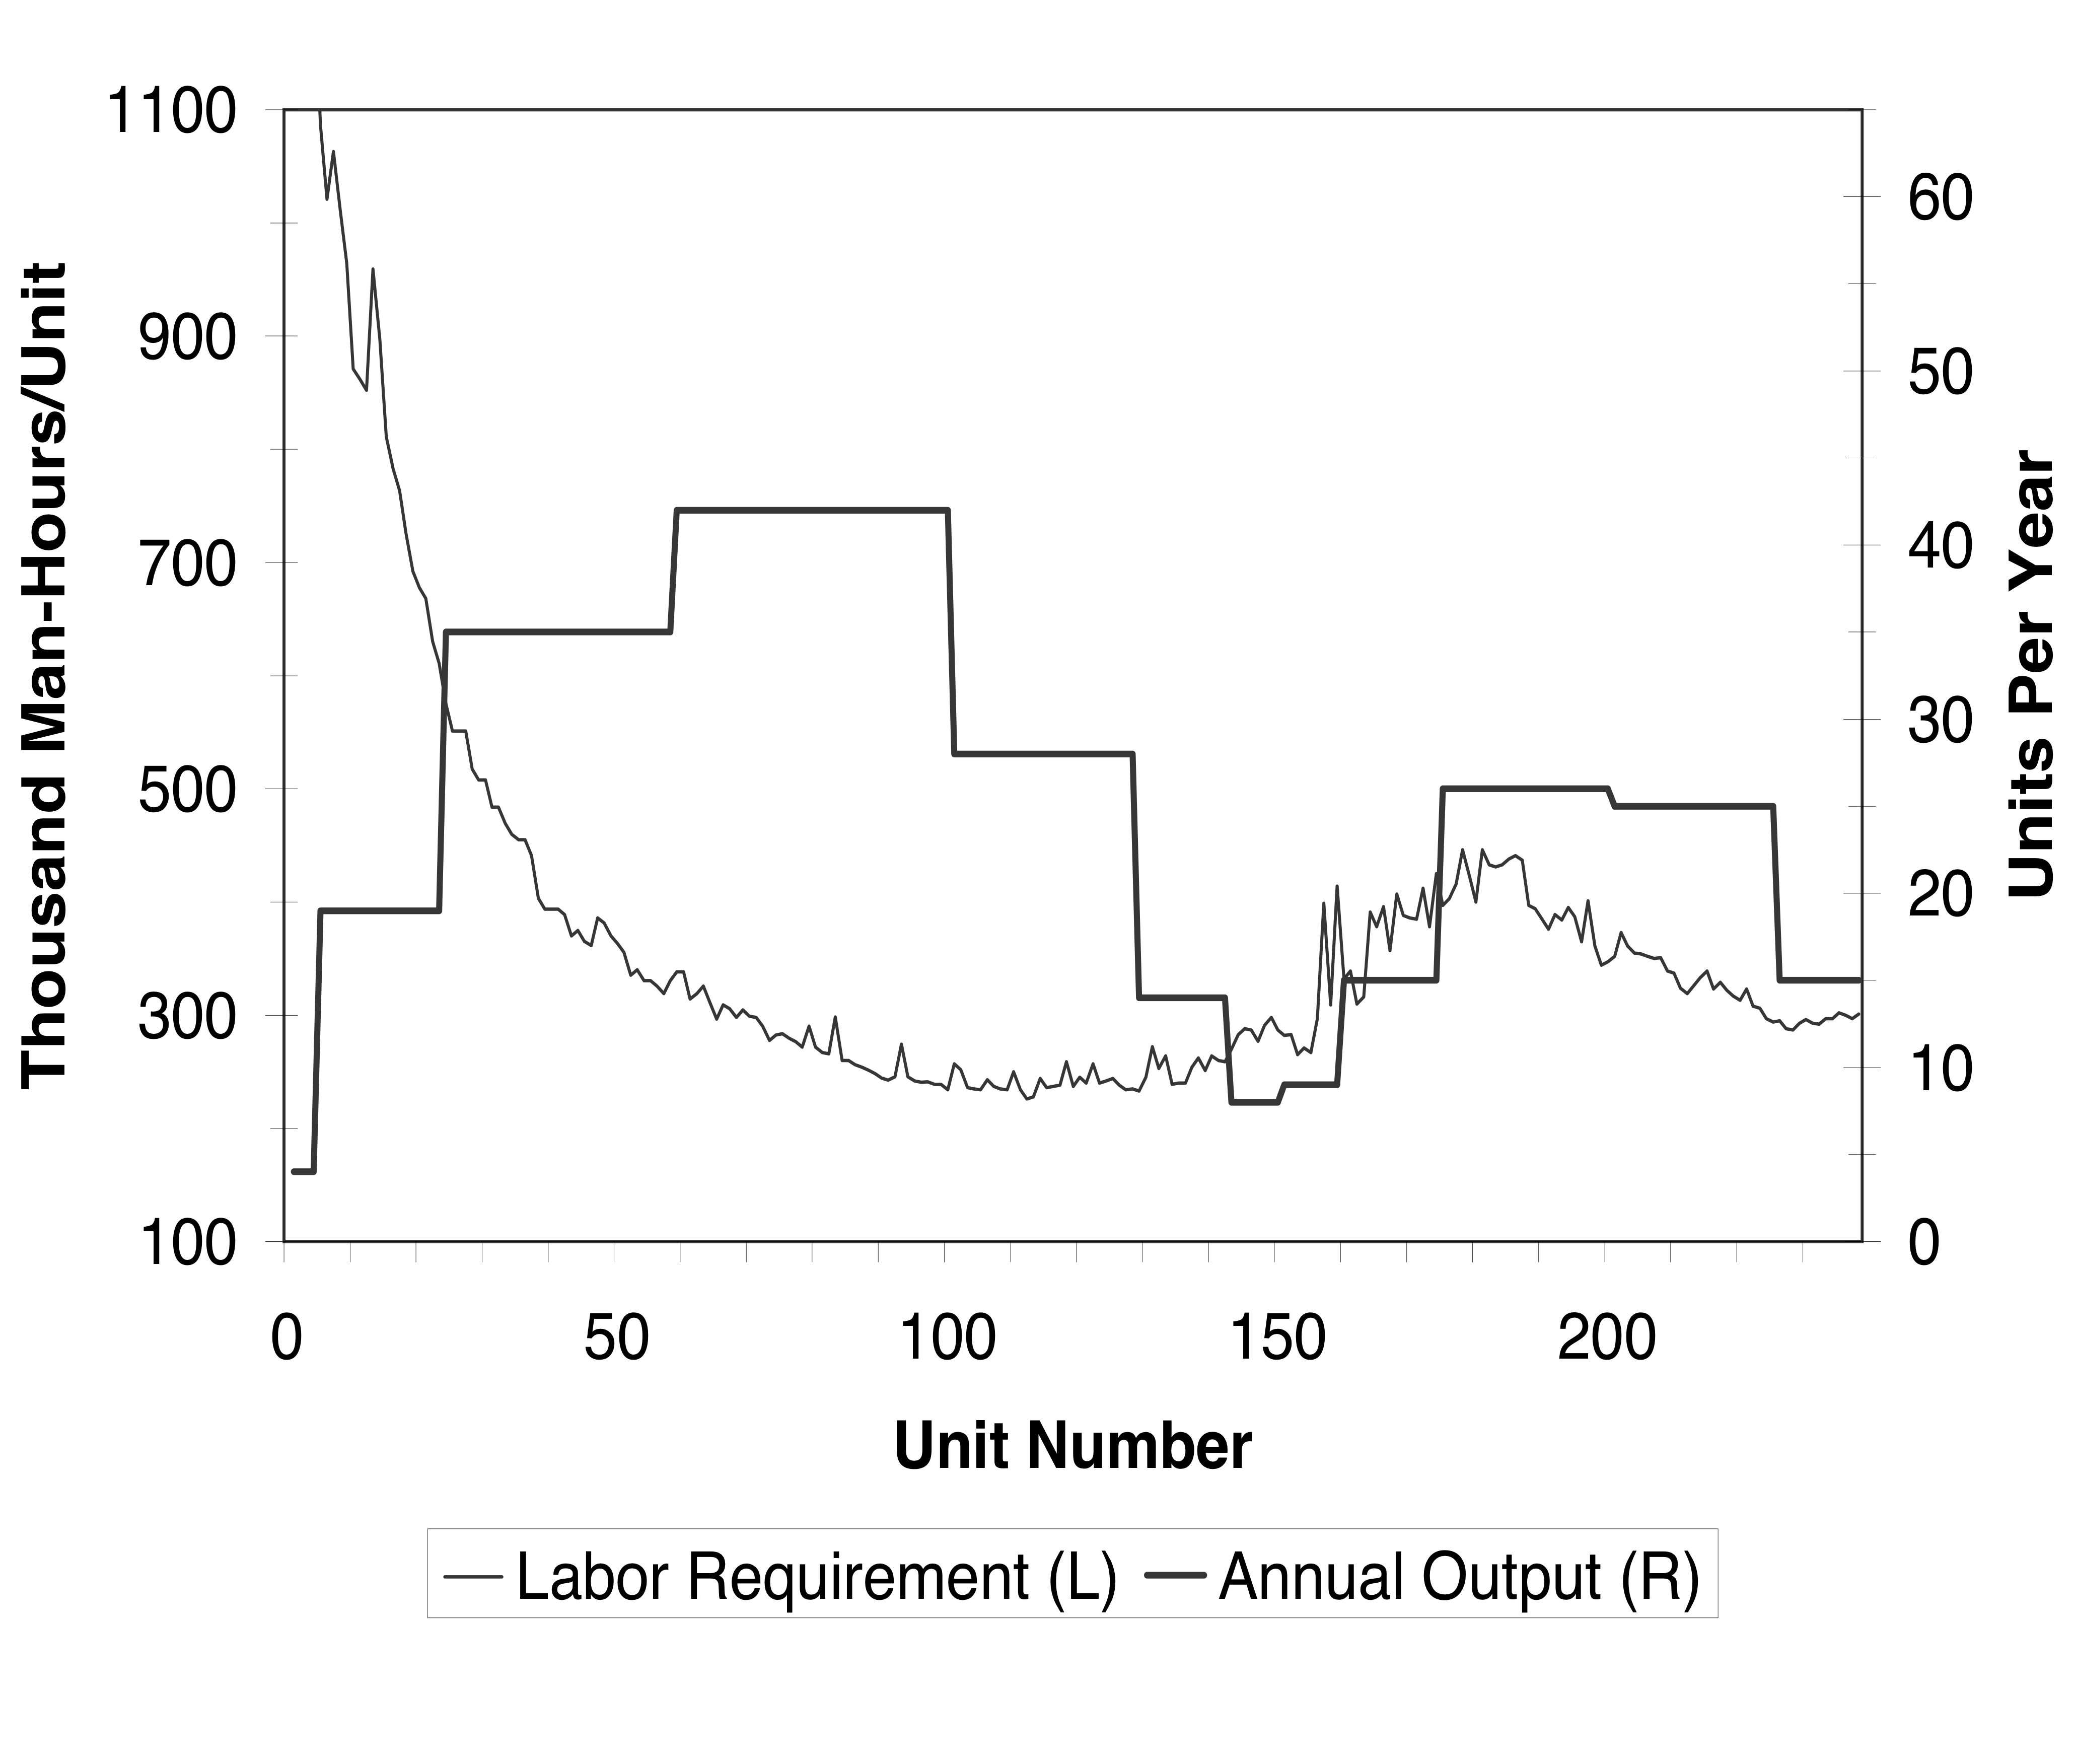
\includegraphics[scale=.43]{learning_and_forgetting.png} 
\end{center}
\end{frame}

%------------------------------------------------------------------------------------------------------------------------------
%------------------------------------------------------------------------------------------------------------------------------


\begin{frame}{Benkard (2000)}
\framesubtitle{Learning and Forgetting: The Dynamics of Aircraft Production} 
\small
Production of complex products may exhibit interesting dynamics
\begin{itemize}\footnotesize
	\item As production ramps us, workers/managers may learn how to streamline processes, make fewer mistakes, spend less time correcting them.
	\item When production decreases, these abilities may diminish if workers are replaced.
\end{itemize}

\vspace{0.5cm}

Interesting implications for returns to scale/scope and product variety
\begin{itemize}\footnotesize
	\item Pricing low at an early stage may improve cost efficiency $\rightarrow$ low-prices are an investment.
	\item Product variety in unconstrained equilibrium may be detrimental to cost efficiency.
\end{itemize}
\end{frame}









\begin{comment}
\begin{frame}[plain]
\footnotesize

\vspace{1.1cm}
\begin{center}
\huge 
\textbf{Demand for Storable Goods}
\end{center}
\end{frame}

\begin{frame}{Demand for Storable Goods}
\vspace{-0.6cm}
\textbf{References:}
\begin{itemize}
    \footnotesize
\item[$-$] Pesendorfer (2002), Erdem, et al. (2003), Hendel and Nevo (2006).
\end{itemize}    

\textbf{Observation:}
\begin{itemize}
\footnotesize
\item[$-$] When a supermarket cuts the price of laundry detergent for a week there is a large increase in sales. This leads us to conclude consumers are extremely elastic with respect to price
\item[$-$] When a supermarket makes a permanent price cut to laundry detergent, there is little sales impact in the long run. Now consumers look highly inelastic with respect to price
\end{itemize}

\textbf{Purchasing vs. consumption elasticity}
\begin{itemize}
\footnotesize
\item[$-$] In the short-run, store-level demand elasticity reflect stockpiling behavior.
\item[$-$] In the long-run, store-level demand elasticity reflects consumption decisions.
\end{itemize}
\footnotesize

\vspace{0.1cm}
$\rightarrow$ Ignoring stockpiling and forward-looking behavior can lead to \textbf{biased own
and cross price elasticities}.

\end{frame}




\begin{frame}{Demand for Storable Goods}{Price discrimination theory of sales:}

\footnotesize
If consumers differ in the storage costs (or credit constraints) firms have an incentive to price
discriminate. Ketchup pricing example (Pesendorfer 2002):

\vspace{-7.0cm}   
\begin{center}
\hbox{
\hspace{-2.0cm}
\includegraphics[scale=.70]{resources/pesendorfer2002.pdf}
}
\end{center}
\end{frame}


\begin{frame}{Hendel and Nevo (2006)}
\textbf{Model:}
\begin{l_itemize}\footnotesize
\item[$-$] A dynamic model of purchase behavior and iventory as a state. 
\end{l_itemize}  

\textbf{Data:}
\begin{l_itemize}
\footnotesize
\item[$-$] Dominick's, 9 Supermarkets in Chicago. \textit{Nielsen Scanner Data}, available through the \textit{Booth Kilts Center}. 
% \item[$-$] Three years of data (1991-1993), store level and household panel. 
\item[$-$] \textbf{Store level:} For each product in each store-week observe average price, average quantity, promotions.
\item[$-$] \textbf{Household level:} Sample of households, supermarket visits, total expenditure during each visit, detailed purchase information in 24 product categories.
\end{l_itemize}
\end{frame}


\begin{frame}{Hendel and Nevo (2006)}
\framesubtitle{Observations from Reduced Form Companion Paper}
\small

\begin{l_itemize}\footnotesize
\item[$-$] Aggregate demand increases as a function of duration from previous sale. 
\item[$-$] Fraction of purchases on sale is higher in markets with larger houses, and if there is a dog in the house. Both of these measures could potentially be correlated with lower storage costs. 
\item[$-$] When buying on sale, households tend to buy more quantity and postpone their next purchase.
\item[$-$]  Inventory is negatively correlated with quantity purchased and the probability of purchase. 
\item[$-$] The patterns of sales across different product categories are consistent with the variation in storage costs across these products. 
\end{l_itemize}
\end{frame}


% \begin{frame}{Hendel and Nevo (2006)}
% \framesubtitle{Consumers have Inventories}
% \begin{itemize}
% \footnotesize
% \item[$-$] Hendel and Nevo suggest that consumers respond by temporary price  reductions by stockpiling inventories.
% \item[$-$] Consumers spend down their inventories during periods of high prices
% \item[$-$] Consumers have variable storage costs and price sensitivities.
% \item[$-$] This has implications for inter temporal price discrimination and retail high-low pricing strategies.
% \end{itemize}
% \end{frame}




% \begin{frame}{Hendel and Nevo (2006)}
% \framesubtitle{Data and Model Basics}
% \begin{itemize} 
% \item[$-$] Store-level: for each brand 13 ($j$) size $x$: 32-256oz in each store, each week ($t$)
% \begin{enumerate}
% \item[$-$] Price $p_{jxt}$ 
% \item[$-$] Quantity $q_{jxt}$
% \item[$-$] Promotions $a_{jxt}$ (binary for feature/display)
% \end{enumerate}
% \item[$-$] Consumers are of type $h$ with utility: $u(c_{ht} + \nu_{ht}; \theta_h)$
% \item[$-$] Current consumption is $c_{ht} = \sum_j c_{jht}$ not brand specific!
% \item[$-$] There is a shock affected marginal utility of consumption $\nu_{ht}$.
% \item[$-$] Decision: $d_{hjxt} = 1$ is a purchase of $h$ of brand $j$ and size $x$ at $t$. (includes outside option $=0$).
% \end{itemize}
% \end{frame}

% \begin{frame}{Hendel and Nevo (2006)}
% \framesubtitle{Quantity Sold}
% \begin{figure}[htbp]
% \begin{center}
% \includegraphics[width=3.8in]{resources/hntable3.pdf}
% \label{gandr1}
% \end{center}
% \end{figure}
% \end{frame}


% \begin{frame}{Hendel and Nevo (2006)}
% \framesubtitle{The Maximization Problem}
% \vspace{-0.3cm}
% \footnotesize
% \begin{eqnarray*}
% V(s_t)&=& \max_{c_h(s_t),d_{jxt}(s_t)} \sum_t \beta^{t-1} E[ u(c_{ht}+\nu_{ht}; \theta_h) - C_h(i_{h,t+1};\theta_h) \\
% &+&\sum_j d_{hjxt} (\alpha_h^p p_{jxt} + \xi_{hjx} + \alpha_h^a a_{jxt} + \epsilon_{hjxt} )| s_t]\\
% i_{h,t+1} &=& i_{ht} + x_{ht} - c_{ht}\\
% \sum_{j,x} d_{hjxt} &=& 1
% \end{eqnarray*}
% \vspace{-0.3cm}
% \begin{itemize}
% \item[$-$] Abuse of notation: $x_{ht}$ is size of the choice
% \item[$-$] $C_h(i; \theta_h)$ is cost of storage
% \item[$-$] $\xi_{hjx}$ captures expected future differences in utility of $x$ units of $j$ \textbf{at time of purchase}. Strange interpretation, but valid as long as: discounting is low, brand-specific differences in utility (but not consumption) enter linearly.
% \end{itemize}
% \end{frame}



% \begin{frame}{Hendel and Nevo (2006)}
% \framesubtitle{Comments on the State}
% \small

% \textbf{State variable:}
% \begin{itemize}\footnotesize
% \item[$-$] $s_t = \{i_t,v_t,\mathbf{p}_t,\mathbf{a}_t,\mathbf{\xi}_t,\epsilon_t\}$.
% \end{itemize}    

% \textbf{Comments:}
% \begin{itemize}\footnotesize
% \item[$-$] State variable $i_t$ is unobserved to the econometrician.
% \item[$-$] Curse of dimensionality: $\{\mathbf{p}_t,\mathbf{a}_t,\mathbf{\xi}_t,\epsilon_t\}$ is a $4 \times 5 \times J$ dimensional matrix.
% \item[$-$] Rust (1987), also has unobserved state variables (i.e. logit
% errors). However, we assumed that it was conditionally independent of
% the observed state and separately additive, which allowed us to work with
% the expected maximum function. \underline{Here}: it is serially correlated and nonseparable.
% \end{itemize}  


% \textbf{Assumptions}
% \begin{itemize}\footnotesize
% \item 1: $\nu_t$ is independently distributed over time and across consumers. \textbf{No serial correlation!}

% \item 2: Prices $p_{jxt}$ and advertising $a_{jxt}$ follow an exogenous first-order Markov process. \textbf{Hard to justify this with a model of profit maximizing supply!}
% \item 3: $\epsilon_{jxt}$ is i.i.d. extreme value type 1.
% \end{itemize}

% \end{frame}



% \begin{frame}{Hendel and Nevo (2006)}
% \framesubtitle{Likelihood}\small
% Conditional on Household we can write the probability of a sequence of purchase decisions. Beginning of period inventory depends on previous decisions, previous shocks, and initial inventory.

% \begin{eqnarray*}
% P(d_{jx} | p_t,i_t,\nu_t) &=& \frac{\exp[\alpha p_{jxt} + \xi_{jx} + \beta a_{jxt} + M(s_t,j,x)]}{\sum_{k,y} \exp[\alpha p_{kyt} + \xi_{jy} + \beta a_{kyt} + M(s_t,k,y)]}\\
% M (s_t,j,x) &=& \max_c [ u(c+\nu_t) - C(i_{t+1}) + \beta E[V(s_{t+1}|d_{jx},c,s_t]]\\
% \end{eqnarray*}

% State space has very \textbf{high dimension}. Keeping track of all brands/prices would be very costly

% \end{frame}

% \begin{frame}{Hendel and Nevo (2006)}
% \framesubtitle{3-Step Proceure}
% To reduce complexity, Hendel and Nevo propose a 3-step estimator
% \begin{itemize}
% \item[$-$] \underline{First}, maximize likelihood of observed brand choice \textbf{conditional} on size in order to recover the $(\alpha,\xi)$ parameters.
% %\item[$-$] This avoids solving MDP but instead is just static discrete choice problem (efficiency loss!)
% \item[$-$] \underline{Second step}: compute \textbf{inclusive values} for each size and transition probability matrix.
% \item[$-$] \underline{Third}, solve a quantity choice only nested fixed point problem. The key is that there is \textbf{only one ``index price'' per size}.
% %\item[$-$] The reason this is feasible is our old friend, the \textbf{conditional independence assumption} (of what?)
% \end{itemize}
% \end{frame}

% \begin{frame}{Hendel and Nevo (2006)}
% \framesubtitle{Step 1: Brand Choice}
% \small
% \begin{equation*}
% P(d_{jx} | p_t,i_t,\nu_t) = \frac{\exp[\alpha p_{jxt} + \xi_{jx} + \beta a_{jxt} + M(s_t,j,x)]}{\sum_{k,y} \exp[\alpha p_{kyt} + \xi_{jy} + \beta a_{kyt} + M(s_t,k,y)]}
% \end{equation*}

% \vspace{0.2cm}

% \begin{equation*}
% M (s_t,j,x) = \max_c [ u(c+\nu_t) - C(i_{t+1}) + \beta E[V(s_{t+1}|d_{jx},c,s_t]]
% \end{equation*}


% \begin{itemize}
% \small
% \item[$-$] The trick is that $M(s_t,j,x)$ is the same for all products of the same size $x$.
% \item[$-$] This means dynamics drop out of the brand-choice equation conditional on $x$.
% \item[$-$] Recover $(\alpha, \xi)$ from static demand estimation:
% \end{itemize}
% \begin{eqnarray*}
% P(d_{jx} | x_t, p_t,i_t,\nu_t) &=& \frac{\exp[\alpha^p p_{jxt} + \xi_{jx} + \alpha^a a_{jxt}]}{\sum_{k,y} \exp[\alpha^p p_{kyt} + \xi_{jy} + \alpha^a a_{kyt}  ] }\\
% &=&P(d_{jx} | x_t, p_t)
% \end{eqnarray*}

% \end{frame}

% \begin{frame}{Hendel and Nevo (2006)}
% \framesubtitle{Step 2: Inclusive Values}
% \small
% \textbf{Assumption 4,} IVS: $F(\omega_t | s_{t-1}) = F(\omega_t | \omega_{t-1})$.

% \begin{equation*}
% \omega_{xt} = \mathbb{E}\big[ \max_j u_j \big] = \log \left( \sum_k \exp(\alpha^p p_{kxt} + \xi_{xt} + \alpha^a a_{kxt}) \right)
% \end{equation*}
% \begin{itemize}\footnotesize
% \item[$-$] Compute ex-ante expected utility of purchasing size $x$ in period $t$
% \item[$-$] Does not depend on which $j$ is purchased.
% \item[$-$] Same as G\&R two price vectors with same inclusive values must have same transition probabilities. Do individual prices still matter? (Test)
% \end{itemize}
% \end{frame}


% \begin{frame}{Hendel and Nevo (2006)}
% \framesubtitle{Step 3: Dynamic Choice of Size}
% \small
% \begin{multline*}
% V(i,\omega_t,\epsilon_t,\nu_t) = \max_{c,x} [ u(c + \nu_t) - C(i_{t+1}) + \omega_{xt} + \epsilon_{xt} + \\
% \beta E[V(i_{t+1},\omega_{t+1},\epsilon_{t+1},\nu_{t+1}) | i_t, \omega_t, \epsilon_t, \nu_t, c, x] ]
% \end{multline*}

% \begin{itemize}\footnotesize
% \item[$-$] Compute ex-ante expected utility of purchasing size $x$ in period $t$
% \item[$-$] Does not depend on which $j$ is purchased.
% \item[$-$] \textbf{IVS} means we can keep track of a lot less information.
% \item[$-$] Same as G\&R two price vectors with same inclusive values must have same transition probabilities.
% \item[$-$] Do individual prices still matter? (Test)
% \end{itemize}
% \end{frame}

% \begin{frame}{Hendel and Nevo (2006)}
% \framesubtitle{Key Proposition}
% \small
% How do we know that the simplified problem has the same solution as the original dynamic problem?
% \begin{eqnarray*}
% P(x_t | i_t,s_t, \nu_t) = P(x_t | i_t, \omega(s_t),\nu_t)
% \end{eqnarray*}

% \begin{itemize}\footnotesize
% \item[$-$] Before we got to see the entire state $s_t$
% \item[$-$] Now we only see the expected utility of $x_t$ aka $\omega_{xt}$
% \item[$-$] The proof relies on Assumption 3(IID Logit errors) and Assumption 4 (IVS).
% \end{itemize}
% \end{frame}

% \begin{frame}{Hendel and Nevo (2006)}
% \framesubtitle{Unobserved initial conditions}
% \textbf{Remaining problem}: $i_t$ is unobserved. \textbf{Solution}: Integrate out the unobserved initial inventory levels.
% \vspace{0.3cm}

% \begin{itemize}\footnotesize
% \item[$-$] Let $i_{i0} = 0$.
% \item[$-$] Simulate the model for the first $T_0$ weeks of the data.
% \item[$-$] Record inventory level at $T_0: i_{T_0}$ (i.e. initial state variable).
% \item[$-$] Evaluate the likelihood from weeks $T_0$ to $T$, as if inventory levels were observed.
% \item[$-$] Repeat the process $S$ times, and average the likelihood contribution
% of individual $i$.
% \item[$-$] \textbf{Implicit assumption}: Stationary process at time $T_0$.
% \end{itemize}
% \end{frame}


% \begin{frame}{Hendel and Nevo (2006)}
% \framesubtitle{Elasticities Compared to Static Model}
% \begin{figure}[htbp]
% \begin{center}
% \includegraphics[width=4.5in]{resources/hntable8_1.pdf}
% \label{gandr1}
% \end{center}
% \end{figure}
% \end{frame}

% \begin{frame}{Hendel and Nevo (2006)}
% \framesubtitle{Elasticities Compared to Static Model}
% \begin{figure}[htbp]
% \begin{center}
% \includegraphics[width=4.8in]{resources/hntable8_2.pdf}
% \label{gandr1}
% \end{center}
% \end{figure}
% \end{frame}








\begin{frame}{Hendel and Nevo (2006)}
\framesubtitle{Important Implications from Comparison with Static Model}
\vspace{-0.3cm}

Two differences between \textit{static} and \textit{dynamic} model: 
\begin{enumerate}\footnotesize
\item Static model implies larger price coefficient,
\item And ignores the inventory problem.
\end{enumerate}
Both points lead to a \underline{larger own price elasticity} with the static model, than the long-run own price elasticity with the dynamic model.

\bigskip 
Point two leads to a \underline{lower cross price elasticity} (compared to static model):
\begin{itemize}\footnotesize
\item[$-$] In the data the response to sales is mostly coming from people going
from not buying to buying the brand on sale.
\item[$-$] This leads to predict small cross price elasticities with respect to other
products, and large cross price elasticity with respect to the outside
good.
\item[$-$] The dynamic model rationalize this phenomenon high unobserved inventories, and conditional choice probabilities (conditional on purchasing).
Everybody needs laundry detergent...
\end{itemize}
\end{frame}


%------------------------------------------------------------------------------------------------------------------------------
%------------------------------------------------------------------------------------------------------------------------------




%------------------------------------------------------------------------------------------------------------------------------
%------------------------------------------------------------------------------------------------------------------------------

\end{comment}



% \begin{frame}{Dynamic Programming}
% \framesubtitle{A Simple Investment Example} 

% \textbf{Primitives:} \\

% \begin{itemize}
% \small 
% 	\item $\pi(\omega_t,x_t,z_t): \Omega \times R \times Z \rightarrow R$. State is $s_t = (\omega_t,z_t).$
% 	\begin{itemize}
% 		\item $\omega$ is the state variable that is affected by \textit{investment} (or some other control), $x_t$, and evolves according to a Markov process $P_{\omega}(\omega_{t+1} \vert \omega_t, x_t)$.
% 		\item $z_t$ are exogenous variables (e.g., input factor costs, demand shocks, etc.). Evolves according to an \textit{exogenous} Markov prcess $P_z(z_{t+1},z_t)$.
		
% 	\end{itemize}
% 	\item Cost of investment $c(x)$
% \end{itemize}

% \textbf{Define objects:} \\

% \begin{itemize}
% \small 
% 	\item History $S^t \equiv (s_1,...,s_t)$
% 	\item Investment policy $\psi \equiv \{ \psi_t(S^t): S^t \rightarrow X \}_t$ . Complicated object.
% \end{itemize}
% \end{frame}



% \begin{frame}{Dynamic Programming}
% \framesubtitle{A Simple Investment Example} 
% \small
% \textbf{Sequence problem}: Objective of decision maker is to choose $\psi \in \Psi(s_1)$ (where $\Psi(\cdot)$ is set of all feasible policies) to maximize the Expected PDV of cash flows:

% \vspace{-0.8cm}

% \begin{align*}
% V_{\psi}(s_1) & = E_{\psi} \big[  \sum_{t=0}^{\infty} \beta^t (\pi(s_t) - c(\psi_t(s^t))) \vert s_1 \big] \\
% & = \sum_{t=0}^{\infty} \beta^t \sum_{s_t} (\pi(s_t) - c(\psi_t (s^t))) p(s_t \vert \psi,s_1)
% \end{align*}

% \vspace{-0.8cm}


% where

% \[ p(s_t \vert \psi,s_1) = \prod_{s_{t-1},...,s_2} p(s_t \vert s_{t-1},\psi_{t-1}(s^{t-1}))...p(s_2 \vert s_1,\psi_1(s^1))\]

% Let 
% \[V^*(s_1) = \sup_{\psi \in \Psi(s_1)} V_{\psi}(s_1)\] 
%  be the value from following the optimal policy in state $s_1$. Problem is to find the optimal policy $\psi^*(s_1)$ for \underline{every possible value $s$}. Seems hard (if not impossible).

% \end{frame}




% \begin{frame}{Dynamic Programming}
% \framesubtitle{The Principle of Optimality}\small

%       \begin{block}{Principle of Optimality}
%         An optimal policy has the property that whatever the initial state and initial decision are, the remaining decisions must constitute an optimal policy with regard to the state resulting from the first decision.
%       \end{block}

% \vspace{0.2cm}

% \textbf{Functional Equation:} Let $s = (w,z).$ Problem can be simplified by expressing the value function from following an optimal policy:

% \begin{equation}
% v(s) = \sup_{x \in X} \{ \pi(s) - c(x) + \beta\cdot \int_{w',z'} v(w',z')\cdot p(w' \vert  w,x) \cdot p(z' \vert z) \} 
% \end{equation}

% \begin{itemize}
% 	\item Note this equation expresses a function in terms of itself (a fixed point).
% 	\item Known as the Bellman equation. Transforms problem into finding a single function.
% \end{itemize}

% \end{frame}



% \begin{frame}{Dynamic Programming}
% \framesubtitle{Solving for the Value Function}\small
% \small

% %\textbf{Solving for the Functional Equation:} \\

% \begin{itemize}
		
% 	\item Stokey and Lucas provide conditions under which solution to (1) equals $V^*(s)$, and any $x(s)$ which solves (3) is an optimal policy for $V^*(\cdot)$.
% 	\item A sufficient condition is that $V^*(\cdot)$ is bounded.

% 	\item This will be a fixed point of the operator $T:B(S)\rightarrow B(S)$ (defined pointwise on space of continuous and bounded real fcts.)

% 	\item Assuming that $\pi(s)$ is bounded, and assuming that $T$ is a contraction mapping (can be proven: c.f. Blackwell (monotinicity, discounting)), can solve for $V^*(s)$ by iterating on (1) from an arbitrary starting point.
% 		\begin{itemize}
% 			\item E.g., let $v^0(s) = \pi(s)$. $v^1(s)$ is value fct. for a two-period problem, and can be solved point-wise. 
% 			\item Practical consideration: control or state variable might be continuous $\rightarrow$ solve on grid, interpolate. 
% 		\end{itemize}

% \end{itemize}
% \end{frame}


\begin{frame}[plain]
\footnotesize
\vspace{1.1cm}
\begin{center}
\huge 
\textbf{Canonical Dynamic Discrete Choice (DDC)}
\end{center}
\end{frame}

\begin{frame}{Dynamic Discrete Choice}
\framesubtitle{Some High Level Comments}

\small

\begin{l_itemize}
\item This literature has a strong focus on computation.
\item The main problem is that the estimation, as in BLP, solves a nested fixed point. 
\item Unlike the demand literature the DDC literature that deals with endogeneity and unobservable confounds is much less developed. 
\item Requires more restrictive assumption than static discrete choice. 
\end{l_itemize}
\end{frame}


\begin{frame}{Outline}
\framesubtitle{Computing/estimating models of dynamic discrete choice.} 
\small
\begin{itemize}\footnotesize
	\item Many economic problems are inherently dynamic: \textit{investment decisions, capacity choice, entry, R\&D, certain types of demand.}
	\item Goal: Correct for \textbf{biases} using static methods in dynamic environments.
	\item Goal: Make more realistic counterfactual predictions.
	\item Surveys: Rust (1994), Aguirregabiria and Mira (2010).
	\item These methods can be used widely across fields!
\end{itemize}
      \begin{block}{Toolbox}\footnotesize
        Nested fixed point estimation (NFXP), conditional choice probabilities (CCP), mathematical programming with equilibrium constraints (MPEC), EM-Algorithm, simulation based estimation, inclusive value sufficiency, linear representation of DDC Model.
      \end{block}
\end{frame}


\begin{frame}{Outline}
\framesubtitle{Road Map for Single Agent Dynamics} 
\vspace{-0.3cm}
\begin{enumerate}\footnotesize
	\item Introduction to canonical dynamic discrete choice (DDC) model, Rust 1994.
	\item DDC Estimation 1 (NFXP): ``Brute Force''. %(\underline{Problem Set 1})
	\item DDC Estimation 2 (CCP): Exploiting observed policies. %(\underline{Problem Set 1})
	\item DDC Estimation 3 (MPEC): Exploiting modern computational methods. 
	\item Identification of DDC models.
	\item DDC and persistent unobserved heterogeneity.
	\item Linear representation of DDC models.		
	\item Simulation based estimation of DDC models.
	\item Applications in dynamic demand: Durable upgrade decisions.		
\end{enumerate}
% \footnotesize
% \textbf{Recitation Friday}: Refresher in dynamic programming, including a practical introduction to solving a McCall model.
\end{frame}

\begin{frame}{Basic model}
\framesubtitle{Canonical Dynamic Discrete Choice}

\small

\begin{itemize}
\item Discrete time $t$, agent $i$, finite or infinite horizon
\item $s_{it}$: vector of state variables
\item $a_{it} \in A = \{0,1,...,J\}$: discrete action
\item Agent's beliefs $F(s_{it+1} \vert s_{it},a_{it})$ (usually Markov and rational expectations (a key identification assumption)).
\item Agent's optimization gives rise to dynamic program:

\begin{equation*}
V(s_{it}) = \max_{a\in A} \{ u(a,s_{it}) + \beta\cdot \int V(s_{it+1})\cdot dF(s_{it+1} \vert s_{it},a) \} 
\end{equation*}

% \item Define the \textbf{choice-specific value function} as:

% \[v(a,s_{it}) = u(a,s_{it}) + \beta \int V(s_{it+1}) dF(s_{it+1} \vert s_{it},a) \]

% \item Then the optimal choice is $\alpha(s_{it}) = argmax_{a\in A} \{ v(a,s_{it})$ \}.
\end{itemize}
\end{frame}

\begin{frame}{Basic model}
\framesubtitle{Data and Primitives}

	\small 
	
	\textbf{Data typically used:}
	
	\begin{itemize}
		\item $N$ individuals forming a panel $(i,t)$.
		\item Observables: actions $a_{it}$, observable state variables $x_{it}$
		\item Unobservables (econometric error): $\epsilon_{it}$.
			\begin{itemize}
				\item This error is ``structural'' in the sense that $s_{it} = (x_{it},\epsilon_{it})$.
			\end{itemize}
	\end{itemize}
	
	\textbf{We may seek to estimate:}
	
	\begin{itemize}
		\item Structural parameters governing preferences in $u(a,s_{it})$.
		\item Transition probabilities.
		\item Discount factor $\beta$ (typically difficult to identify, more on this later).
	\end{itemize}
	
\end{frame}


\frame {
	\frametitle{Dynamic Programming}
	\framesubtitle{Assumptions on unobservables}
	\small

\begin{itemize}
	\item \textbf{Additive separability}:
		\begin{itemize}
			\item $u(a,x_{it},\epsilon_{it}) = u(a,x_{it}) + \epsilon_{it}(a)$. 
			\item One unobservable for each action, so dimensionality of $\epsilon_{it}$ is $J \times 1$. 
      %$\theta_U$ represents parameters governing $u$ and $G_\epsilon$.
		\end{itemize}
	\item \textbf{Type-I Extreme Value (logit) errors}
		\begin{itemize}
			\item The unobservable shocks $\{\epsilon_{it}(a), a=1,2,...,J\}$ are independently distributed as Type-I E.V.
		\end{itemize}
	\item \textbf{IID}: 
		\begin{itemize}
			\item $\epsilon$ is i.i.d. distributed over agents and time according to $G_{\epsilon}$.
		\end{itemize}
	\item \textbf{Conditional independence of $x_{it}$}: 
		\begin{itemize}
			\item $F(s_{it+1} \vert s_{it},a) = F(x_{it+1} \vert x_{it},a)\cdot G_{\epsilon}.$ %Governed by $\theta_f$
		\end{itemize}
	
\end{itemize}


\centering
%\hspace{-2mm} %\includegraphics[scale=.4]{Farinas_Ruano_2005_fig1.pdf} 
	
}	


\begin{frame}[plain]
\footnotesize
\vspace{1.1cm}
\begin{center}
\huge 
\textbf{John Rust (1987)}
\end{center}
\end{frame}



\begin{frame}{John Rust (1987)}
\framesubtitle{Harold Zurcher's Problem}

\vspace{-0.4cm}
\begin{itemize}
	\small
	\item He is the superintendent of maintenance at the Madison, WI Metropolitan Bus Company.
	\item Each week, must decide to replace engine or keep running for another week.
	\item This is an \textbf{optimal stopping} problem:
		\begin{itemize}
			\footnotesize
			\item Fixed costs of repair, but new engine has lower future maintenance costs.
			\item Engine maintenance costs grows as engine gets older.
		\end{itemize}
	\item Can show that there is a \textbf{cutoff} mileage threshold $x^*$ above which a bus will have its engine replaced. Common type of optimal policy in many models, for example, job search.

	\item \small Note: as econometricians we are making a very strong assumption, namely that we observe the optimal \textit{solution} to a complex dynamic problem. We want to learn the primitives governing the problem.

	% \item Acknowledgments: ``I am especially grateful to Harold Zurcher for providing the data used in this study, and for his assistance in interpreting the estimation results.'' :-)
\end{itemize}

\end{frame}


\frame {
	\frametitle{John Rust (1987)}
	\framesubtitle{Some Comments}
	\small

\vspace{-0.4cm}

\textbf{Many of the empirical IO appeals, issues, and trade-offs showcased.}
\begin{l_itemize}\small 
	\item Paper about one guy, who cares? The \textit{yogurt/cereals} critique. 
	\item Obviously, this is a paper about methodology, like many early empirical IO papers. \textit{Recently the empirical IO literature has moved away from pure methodological work...}
	\item Model focuses on one particular decision and leaves out many related decisions that Harold Zurcher makes. \textbf{George E.P. Box:} \textit{All models are wrong but some are useful...}
	\item However, your model should capture the crucial aspects that are material to the question. How do omitted aspects affect the conclusions drawn from the paper? It is good practice to think about all model assumptions in light of their effect on counterfactual results.
\end{l_itemize}
}


\frame {
	\frametitle{John Rust (1987)}
	\framesubtitle{Model}
	\vspace{-0.2cm}
\begin{itemize}
	\small
	\item $\theta_1$: parameters of cost function and RC; $\theta_2$: parameters of distribution $\epsilon$ (assumed to be known); $\theta_3$: parameters that govern state transition;$\beta$ imputed. 
	\item $a_t = 1$ if engine is replaced at time $t$, otherwise $=0$. Choose sequence of actions $a \equiv \{ a_1,a_2,...,a_t,...\}$:
	\vspace{-0.2cm}
	\[\max_a E \sum_{t=1}^{\infty} \beta^{t-1} u(x_t,\epsilon_t,a_t; \theta) \]
	\item Mileage $x_{t+1}$ evolves according to $F(x_{t+1} \vert x_t; \theta_3)$ if $a_t=0$, otherwise $x_{t+1}=0$ (engine is brand new if replaced). This transition process can be estimated separately from the model. 
	\item Utility is parameterized $u(x_t,\epsilon_t,a_t;\theta_1,RC) = -c(x_t \cdot (1-a_t); \theta) - a_t \cdot RC + \epsilon_t(a_t)$, where RC is replacement cost and $c$ is increasing in $x_t$.
	\item Want to estimate: parameters of cost function $c$, replacement cost $RC$, and parameters governing $F(x_{t+1} \vert x_t; \theta_3)$.	
\end{itemize}

}

\frame {
	\frametitle{Rust (1987): Data \& Likelihood}
	\framesubtitle{Conditional Independence Assumption}
	\small

Allows to simplify \textbf{transition probabilities} and \textbf{value function}:
 \begin{itemize}
\item Factor transition probabilities: $P(x_{t+1},\epsilon_{t+1} \vert x_t, \epsilon_t,a_t;\theta)=P(x_{t+1}\vert x_t,a_t,\theta_3)\cdot G(\epsilon_{t+1}|x_{t+1},\theta_2)$
\item Do not need to treat unobserved $\epsilon$'s as state variables. Can write $EV_\theta (x_t,a_t)$ instead of $EV_\theta (x_t,\epsilon_t,a_t)$. Can express Bellman eq. in terms of EV. 
\item \underline{Testable:} estimate alternative model where last periods decision enters utility, then perform likelihood ratio test. 
\end{itemize}

\vspace{0.5em}

Also, with \textbf{CI} the \textbf{likelihood function} can be simplified to:
\begin{equation*}
 \log \ell(x_1,...,x_T,a_1,...,a_T \vert x_0,a_0 ; \theta) =
 \sum_{t=1}^T \log F(x_t \vert x_{t-1},a_{t-1};\theta_3) + \sum_{t=1}^T \log P(a_t\vert x_t;\theta_1)
 \end{equation*}
 \vspace{-0.5em}
\begin{itemize}
\item Two components: the mileage transitions, and the probability of replacement.
 \end{itemize}
}


\frame {
	\frametitle{Rust (1987)}
	\framesubtitle{Comments on the Specification}
	\small

The likelihood function is not specified directly. 
\begin{itemize}\footnotesize
\item Instead, it is \textit{derived} from the solution to the underlying optimization problem
\end{itemize}

Rust distinguishes structural model from reduced form:

\begin{itemize}
	\footnotesize
	\item The parametric specification occurs at the level of the primitive objects of the model (utility function and transition probabilities).
\end{itemize}	

He discusses the importance of incorporating unobservables into the dynamic optimization:

\begin{itemize}
	\footnotesize
	\item Model without ``error term'': due to cut-off rule in $x_t$ model would be immediately rejected by the data. 
	\item Econometric model where error term is simply added to the model solution lacks interpretation. Instead, view $\epsilon_t$ as a state variable which is unobserved to the econometrician but observed by agents (enters utility function).
\end{itemize}
}	


% \frame {
% 	\frametitle{Rust (1987)}
% 	\framesubtitle{Theorem 1}

% \begin{block}{Theorem 1}
% \footnotesize
% Given CI:

% \begin{equation*}
% P(a|x,\theta) = \frac{\partial}{\partial u(x,a,\theta_1)}\cdot G\big(u(x,\theta_1) + \beta \cdot EV_\theta (x) \vert x,\theta_2 \big)
% \end{equation*}
% where $EV_\theta$ is the unique fixed point to the contraction mapping:

% \begin{equation*}
% EV_\theta (x,a) = \displaystyle\int_y  G\big(u(x,\theta_1) + \beta \cdot EV_\theta (y) \vert y,\theta_2 \big)\cdot p(dy|x,a,\theta_3)
% \end{equation*}

% and 

% \begin{itemize}
% 	\footnotesize
% \item $P(a|x,\theta)$ is the probability of action $a$ conditional on state $x$.
% \item $G(.|x,\theta_2)$ is the social surplus function: 
% \end{itemize}

% \begin{equation*}
% G(v\vert x,\theta_2) \equiv \displaystyle\int_\epsilon \max_a \Big\{ v(a)+\epsilon(a) \Big\}\cdot q(d\epsilon\vert x,\theta_2)
% \end{equation*}

% \end{block}

% }


% \frame {
% 	\frametitle{Rust (1987): Comments}
% \framesubtitle{}	
% 	\small
% Rust distinguishes structural model from reduced form:

% \begin{itemize}
% 	\footnotesize
% 	\item The parametric specification occurs at the level of the primitive objects of the model
% 		\begin{itemize}
% 			\footnotesize
% 			\item Namely, the utility function and transition probabilities
% 		\end{itemize}
% 	\item The likelihood function is not specified directly, but rather is \textit{derived} from the solution to the underlying optimization problem.
% \end{itemize}	

% Nowadays, Rust (1987) often used as a straw man for computational inefficiency. 
% \begin{itemize}
% \footnotesize

% \item The likelihood function is not specified directly, but rather is \textit{derived} from the solution to the underlying optimization problem
% \item Requires nested fixed point computation (NFXP).

% \item That we solve some economic problem before evaluationg objective function seems trivial now but novel at the time. 


% \end{itemize}
	
% }	







% \frame{
% 	\frametitle{Rust (1987): Estimation}
% 	\framesubtitle{Estimate mileage transition probabilities}
% \small


% \vspace{-0.5cm}

% \textbf{Begin with} $F(x_{t+1} \vert x_t; \theta_3)$.

% \vspace{0.2cm}

% \begin{itemize}\footnotesize
% \item This part of the estimation can be done ``offline''.
%  \item Rust assumes $\Delta x_{t+1} \equiv x_{t+1} - x_t$ follows a discrete multinomial distribution
% \[ \Delta x_{t+1}=\begin{cases}
% \begin{array}{c}
% [0,5000)\\{}
% [5000,10000]\\{}
% [10000,\infty)
% \end{array} & \begin{array}{l}
% \text{with prob }\theta_{3^{0}}\\
% \text{with prob }\theta_{3^{1}}\\
% \text{with prob }1-\theta_{3^{0}}-\theta_{3^{1}}
% \end{array}\end{cases} \]
% \item Can be done first (e.g., using the empirical frequencies in the data)
% \item Space (i.e., milage) is discretized into 90 intervals of length 5,000.
% \end{itemize}
% }




\begin{frame}[plain]
\footnotesize

\vspace{1.1cm}
\begin{center}
\huge 
\textbf{Nested Fixed Point Algorithm}
\end{center}
\end{frame}





\frame{
	\frametitle{Rust (1987): Estimation}
 \framesubtitle{NFXP 1}

\textbf{Key idea:} Estimation first solves an inner ``loop'' (the value function) and then an outer ``loop'', the objective function. Hence, nested fixed point. 

	\centering
\vspace{-0.8cm}
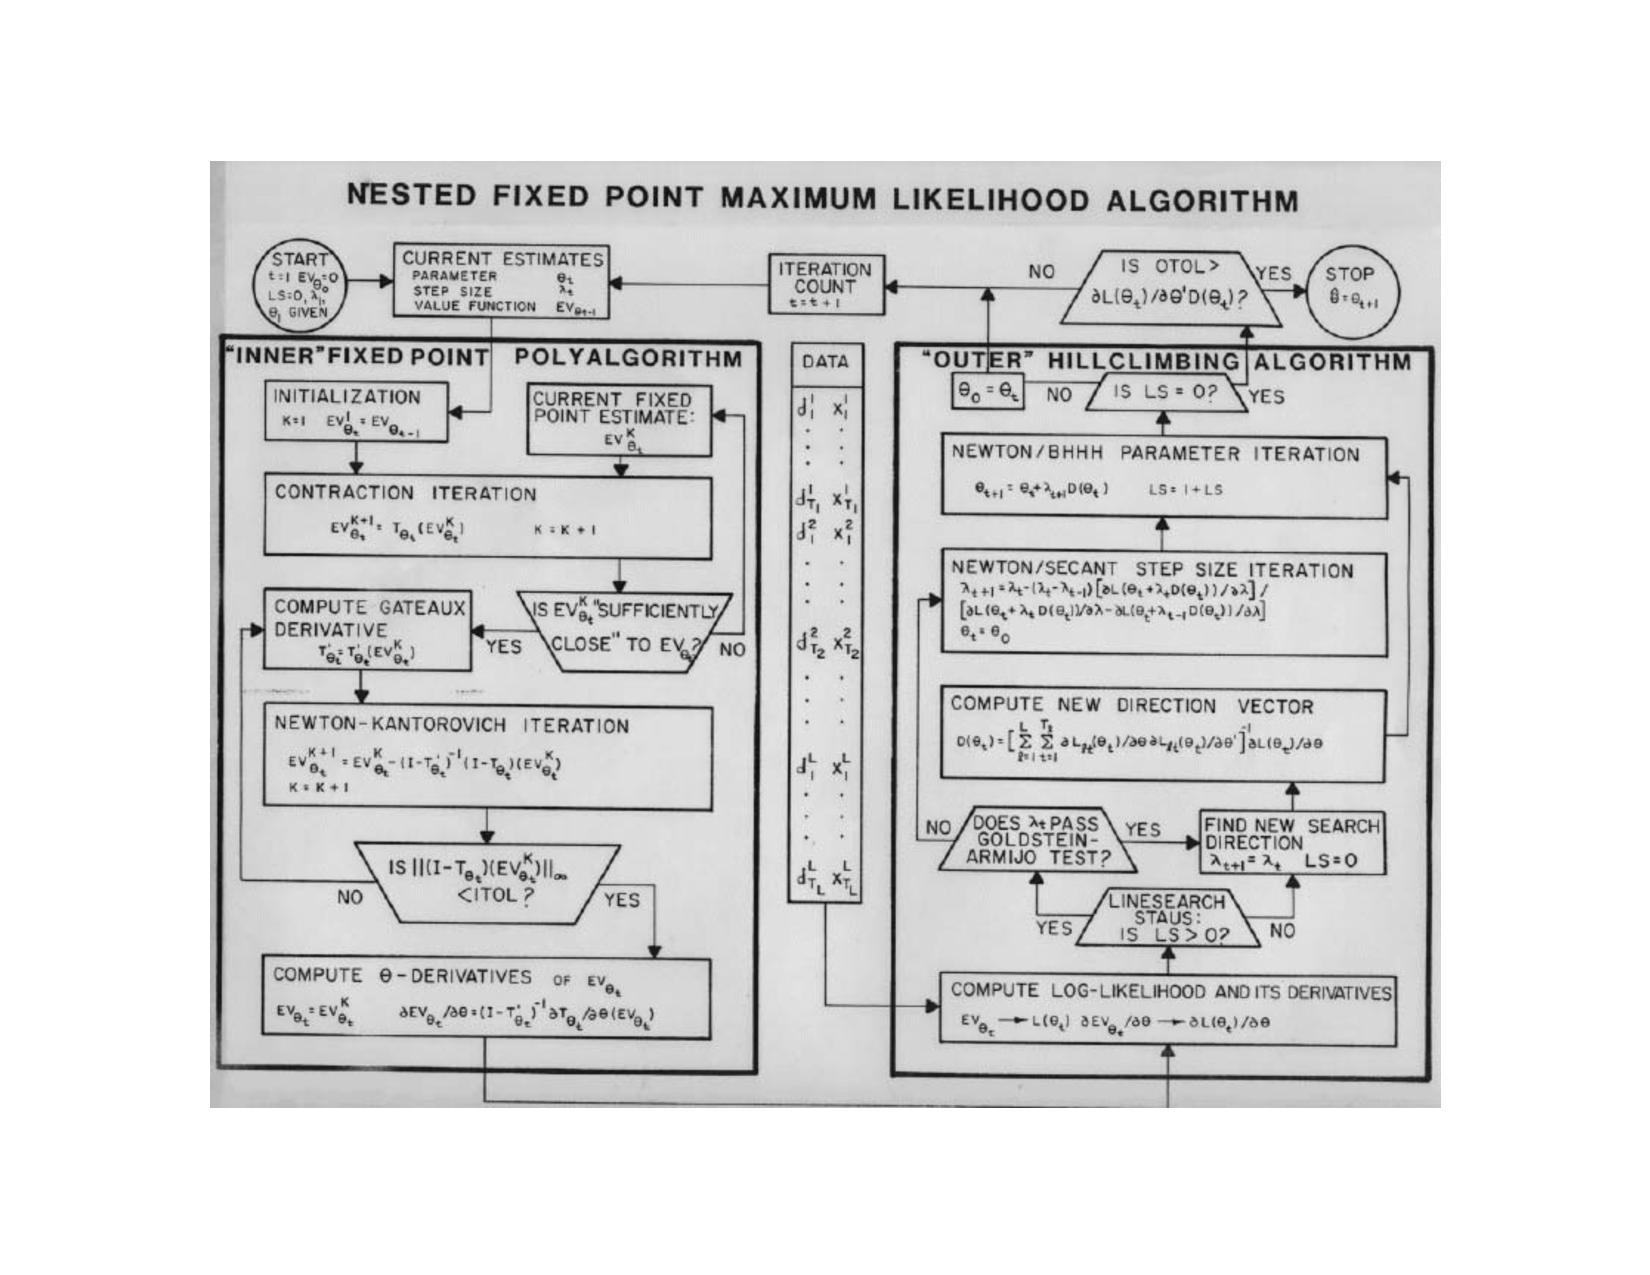
\includegraphics[scale=.38]{nfxp_picture}
	
}





\frame{
	\frametitle{Rust (1987): Estimation}
 \framesubtitle{NFXP 2}
\footnotesize

\vspace{-0.3cm}
\begin{itemize}
\item Note we can specify each agent's dynamic decision problem:
\vspace{-0.3cm}
\[a^\star_t = argmax_a \{ u(x_t,\epsilon_t,a;\theta)+\beta\cdot  EV_\theta(x_t,a)\} \]

\item Let $u(x,a;\theta) \equiv u(x,\epsilon,a;\theta)-\epsilon_a$ be part of the utility minus the error term.

\item Then the \textbf{choice specific value functions} are defined as:
\vspace{-0.3cm}
\begin{equation*}
v_\theta(a,x) \equiv u(x,a;\theta_1)+\beta \cdot EV_\theta (x,a)
\end{equation*}
% \item Recall, utility is parameterized as:

% \[ u(x_t,\epsilon_t,a_t;\theta_1) = -c(x_t (1-a_t);\theta_1)-a_t \cdot RC + \epsilon_{a,t} \]


\item Since we assume that $\epsilon$ are i.i.d. logit:
\vspace{-0.3cm}
\begin{equation*}
P(a_t \vert x_t; \theta_1) = \frac{exp(u(x_t,a_t;\theta_1) + \beta EV_\theta(x_t,a_t))}{\sum_{j=0,1}exp(u(x_t,a_j;\theta_1)+\beta EV_\theta(x_t,a_t))} = \frac{exp(v_\theta(a_t,x_t))}{\sum_{j=0,1}exp(v_\theta(a_j,x_t))}
\end{equation*}

This means that if we can solve for each agent's value function $V_\theta (\cdot)$, we can compute $P(a_t \vert x_t; \theta)$, and form the likelihood.


\end{itemize}
}


\frame{
	\frametitle{Rust (1987): Estimation}
	\framesubtitle{NFXP 3}
\small

For a given parameter value $\theta$ Rust iterates on the \underline{expected value function}.  
	\begin{itemize}
		\item Let $x,a$ denote last period's mileage and choice.
		\item Let $y,j$ denote next period's mileage  and choice.
\vspace{-0.1cm}
\begin{align*}
EV_\theta(x,a) &= E_{y,\epsilon} [V_\theta(y,\epsilon \vert x,a)] \\
&= E_{y,\epsilon}  \big[ \max_{j=0,1} [u(y,j;\theta) + \epsilon + \beta\cdot EV_\theta(y,j)] \big] \\
&= E_y \log \big[  \sum_{j=0,1} exp(u(y,j;\theta) + \beta\cdot EV_\theta(y,j)) \big]
\end{align*}

%where $EV(\cdot)$ is solved for a discretized grid of points $r$ and is interpolated to obtain values on points $x \notin r$.
\item Don't need to evaluate the value function for a grid of the $\epsilon$ draws. 
\item Works because of \textbf{conditional independence} assumption!
\item Once convergence on $EV(\cdot)$ is obtained, the choice probabilities are obtained (as on the previous slide).


\end{itemize}

}


% \frame {
% 	\frametitle{Rust (1987): Estimation}
%  \framesubtitle{NFXP 4}	
% 	\small
% \vspace{-0.2cm}
% \begin{itemize}
% \footnotesize

% \item In practice, Rust uses a combination of a standard \textbf{contraction mapping} and the \textbf{Newton-Kantorovich} algorithm for the inner loop. The latter makes use of the fact that the contraction mapping can be transformed into a root finding problem:

% \[E V_{\theta}=T_{\theta}\left(E V_{\theta}\right) \text{ iff  } \left[I-T_{\theta}\right]\left(E V_{\theta}\right)=0\]

% \item A Taylor series expansion leads to: 
% \vspace{-0.2cm}
% \begin{equation}
% 0=\left[I-T_{\theta}\right]\left(E V_{k+1}\right) \sim\left[I-T_{\theta}\right]\left(E V_{k}\right)+\left[I-T_{\theta}^{\prime}\right]\left(E V_{k+1}-E V_{k}\right)
% \end{equation}

% and therefore: 

% \begin{equation*}
% E V_{k+1}=E V_{k}-\left[I-T_{\theta}^{\prime}\right]^{-1}\left(I-T_{\theta}\right)\left(E V_{k}\right)
% \end{equation*}

% \item Standard contraction mapping is slow, especially for later rounds of the iteration and $\beta$ close to one. Newton-Kantorovich is faster but can be unstable far away from the solution. Rust starts with a few rounds of contraction and then switches to Newton-Kantorovich. 
% \end{itemize}
	
% }	

\frame{
	\frametitle{Rust (1987): Estimation}
	\framesubtitle{Recap and Comments}
\small

\vspace{-0.2cm}
\textbf{Estimation Steps:}
\begin{itemize}\scriptsize
	\item ``Although the data clearly reject the myopic model, I was not able to precisely estimate the discount factor $\beta$.'' Impute value for discount factor. 
	\item Estimate $\theta_3$ $-$ transition function for mileage $-$ can be done without behavioral model 
	\item NFXP outer ``loop'': search over $(\theta_1,RC)$ to maximize likelihood function.
	\item NFXP inner ``loop'': for evaluating a likelihood for a given $(\theta_1,RC)$ need to find fixed point of bellman equation.
\end{itemize}	

\vspace{-0.2cm}
\textbf{Comments:}
\begin{itemize}\scriptsize
	\item Heavy reliance on assumptions, particularly i.i.d. errors and conditional independence of state variables. Discrete states and actions, correct expectations. Will limit certain applications. 
	\item Computationally costly: This is a full-solution method: for every evaluation of the parameter vector $\theta_1$, the agent's dynamic programming problem is explicitly solved (value-function iteration).
	\item Inherits all positive aspects of maximum likelihood. Asymptotically efficient full information estimator.
\end{itemize}
}


\begin{frame}[plain]
\footnotesize

\vspace{1.1cm}
\begin{center}
\huge 
\textbf{Hotz and Miller (1993)} \\
+ \\
\textbf{Hotz, Miller, Sanders and Smith (1994)}
\end{center}
\end{frame}


\frame{
	\frametitle{Estimation: An alternative approach (CCP)}
\framesubtitle{Idea}
\small

\textbf{Key insight:} we can express the value functions in terms of observed choice probabilities. This allows us to obtain the value function without having to solve the agent's optimization problem. This leads to an estimator that is:

\begin{itemize}
\item Computationally efficient but \textbf{not} econometrically efficient.
\item How the mapping from choice probabilities to values is done depends on the application. 
\end{itemize}	

\begin{block}{Important idea}
We don't need to solve for policies whose state variables and outcomes are observed in the data.
\end{block}


}

\frame{
	\frametitle{Estimation: An alternative approach (CCP)}
\framesubtitle{Hotz \& Miller inversion with logit errors }
\small

Let $G(.|x,\theta)$ be the social surplus function: 

\begin{equation*}
G(v\vert x,\theta) \equiv \displaystyle\int_\epsilon \max_a \Big\{ v(a)+\epsilon(a) \Big\}\cdot q(d\epsilon\vert x,\theta)
\end{equation*}

\textit{Theorem 1} in \textbf{Rust (1987)}: 

\begin{equation*}
P(a|x,\theta) = \frac{\partial}{\partial u(x,a,\theta)}\cdot G\big(u(x,\theta) + \beta \cdot EV_\theta (x) \vert x,\theta \big)
\end{equation*}

where: 

\begin{itemize}
\item $P(a|x,\theta)$ is the probability of action $a$ conditional on state $x$.
\end{itemize}


\vspace{0.2cm}

Mapping from \textbf{choice-specific values} to \textbf{choice probabilities}.
}

\frame{
	\frametitle{Estimation: An alternative approach (CCP)}
\framesubtitle{Hotz and Miller (1993) and Hotz, Miller, Sanders and Smith (1994)}
\small

% \textbf{Rather than solve the DP for each value of $\theta$, use idea from :}

\begin{itemize}
\item Notice that CCP's are unchanged when subtracting a constant from every value:
\begin{equation*}
dv(x,a) \equiv v_\theta(x,a) - v_\theta(x,0), 
\end{equation*}
where $a=0$ is some reference action.

\item Let $Q:\mathbb{R}^{\vert \mathbf{J} \vert -1} \rightarrow \Delta^{\vert \mathbf{J} \vert} $ be the mapping from the deltas in conditional values to CCP's.

\item We maintain the assumption that the $\epsilon$ are iid.

\end{itemize}

\begin{block}{Hotz and Miller (1993) Proposition 1}
Q is invertible.
\end{block}

% With logit errors: 
% \begin{equation*}
% Q^{-1}(P) = log(P(a \vert x; \theta)) - log(P(0 \vert x; \theta)) = v_\theta(x,a) - v_\theta(x,0)
% \end{equation*}

}





\frame{
	\frametitle{Estimation: An alternative approach (CCP)}
\framesubtitle{Hotz \& Miller inversion with logit errors  }
\small

Like in Rust, consider $\epsilon \sim$ T1EV, IID. Expression for CCP's:

\[ P(a \vert x; \theta) =  \frac{exp(v_\theta(a,x))}{\sum_{a \in \mathcal{A}}exp(v_\theta(a,x))} \]

The \textit{HM inversion} follows by taking logs and differencing. Thus, with logit errors: 

\begin{equation*}
Q^{-1}(P) = v_\theta(x,a) - v_\theta(x,0)
\end{equation*}




}



\frame{
	\frametitle{Estimation: An alternative approach (CCP)}
\framesubtitle{Using Inversion for Estimation}
\small

The \textbf{inversion result} can be used for estimation in a number ways:

\begin{enumerate}
\item Forward simulation. \textit{Hotz, et Al. (1994)}
\item Finite dependence. \textit{Scott (2016).}
\item Solve a system of equations to express the vector of values in terms of probabilities and parameters. Pesendorfer and Schmidt-Dengler (2008) for dynamic games. 
\end{enumerate}	

	We will now discuss simulation and leave the former approach for when we discuss dynamic games. For both approaches we \textbf{first} need choice probabilities and transition laws:

\begin{equation*}
F(x'\vert x,a)=\begin{cases}
\begin{array}{c}
\sum_{i=1}^{N}\sum_{t=1}^{T-1}\frac{\mathbf{1}(x_{i,t+1}<x',x_{it}=x,a_{it}=0)}{\mathbf{1}(x_{it}=x,a_{it}=0)}\\
\sum_{i=1}^{N}\sum_{t=1}^{T-1}\frac{\mathbf{1}(x_{i,t+1}<x',a_{it}=1)}{\mathbf{1}(a_{it}=1)}
\end{array} & \begin{array}{c}
\text{if }a=0\\
\text{if }a=1
\end{array}\end{cases} 
\end{equation*}

\begin{equation*}
\hat{P}(a=1\vert x)\equiv\sum_{i=1}^{N}\sum_{t=1}^{T}\frac{\mathbf{1}(a_{it}=1,x_{it}=x)}{\mathbf{1}(x_{it}=x)}, \;\;\;\;\;\; \hat{P}(a=0\vert x)\equiv1-\hat{P}(a=1\vert x) 
\end{equation*}

}


\frame{
  \frametitle{Estimation: An alternative approach (CCP)}
\framesubtitle{Forward Simulation}
\small

If $\epsilon$ is i.i.d. logit, then $\mathbb{E}[\epsilon \vert a=a^{*},x] = \gamma - \log(P(a\vert x))$, where $\gamma$ is Euler's constant. 

\begin{equation*}
\mathbb{E}\Big(u(a) + \varepsilon(a) \Big\vert u, a=a^{*}\Big)= \ln \Big(\sum_{j \in J} exp(u(a_j))\Big)+\gamma \Leftrightarrow
\end{equation*}

\begin{equation*}
\mathbb{E}\Big(\varepsilon(a) \Big\vert u, a=a^{*}\Big)= \ln \Big(\sum_{j \in J} exp(u(a_j))\Big) - u(a) +\gamma = \gamma - \log(P(a\vert x))
\end{equation*}

For more algebra tricks for discrete choice have a look at \textit{Discrete Choice Theory of Product Differentiation} by \textbf{Anderson, de Palma, and Thisse}.

}



\frame{
	\frametitle{Estimation: An alternative approach (CCP)}
\framesubtitle{Forward Simulation}
\small

With estimates of $\hat{F}(x'\vert x,a),\hat{P}(a=1\vert x),\hat{P}(a=0\vert x)$ in hand, we can express the choice specific value function (w/o $\epsilon$) for any $a$ taken this period as follows:
\begin{multline*}
v_\theta(a_t,x_t)=u(x_t,a_t;\theta)+ \beta\cdot \mathbb{E}\Big[ u(x_{t+1},a_{t+1};\theta)+\epsilon_{t+1}+ \\
\beta\cdot \mathbb{E} [u(x_{t+1},a_{t+1};\theta)+\epsilon_{t+2}+\beta^{2}\cdot \mathbb{E}[...]]\Big]
\end{multline*}
where expectations are conditional, i.e., the first expectation is $$\mathbb{E}_{x_{t+1}\vert x_t,a_t} \mathbb{E}_{a_{t+1}\vert x_{t+1}} \mathbb{E}_{\epsilon_{t+1}\vert x_{t+1},a_{t+1}}.$$

}



\frame{
	\frametitle{Estimation: An alternative approach (CCP)}
\vspace{-0.5cm}
\begin{itemize}
\small
\item So, for a given $\theta$, simulate forward (for $a=0,1$):
\footnotesize
\begin{multline*}
v_\theta(a,x)\equiv\frac{1}{S}\sum_{s} \left[ u(a,x;\theta)+\beta \cdot \left[ u(a_{t+1}^{s},x_{t+1}^{s};\theta)+ \gamma-\log(\hat{P}(a_{t+1}^{s}\vert x_{t+1}^{s}))+  \right. \right. \\
\left. \left. \beta \cdot [u(a_{t+2}^{s},x_{t+2}^{s};\theta)+\gamma-\log(\hat{P}(a_{t+2}^{s}\vert x_{t+2}^{s}))+\beta \cdot...] \right] \right]
\end{multline*}
\small
\vspace{-0.3cm}

where 

\vspace{-0.3cm}
\footnotesize
\[
x_{t+1}^{s}\sim\hat{F}(\cdot\vert x_t,a_t),a_{t+1}^{s}\sim\hat{P}(\cdot\vert x_{t+1}^{s}),x_{t+2}^{s}\sim\hat{F}(\cdot\vert x_{t+1}^{s},a_{t+1}^{s}),...
\]
\small
\item Given simulated choice-specific value functions, predict CCP's:

\footnotesize
\[ \tilde{P}(a=1\vert x;\theta)\equiv\frac{\exp(v_\theta(a=1,x))}{\exp(v_\theta(a=0,x))+\exp(v_\theta(a=1,x))} \]

\vspace{-0.3cm}
\begin{equation*}\footnotesize
\hat{\theta}=argmin_{\theta}||\left[\log(\hat{P}(a=1\vert x))-\log(\hat{P}(a=0\vert x))\right] -\left[v_\theta(a=1,x)-v_\theta(a=0,x)\right]|| 
\end{equation*}

\end{itemize}
}




\frame{
	\frametitle{Aguirregabiria and Mira (2002)}
\framesubtitle{From Two-Step to K-Step estimators}

The CCP approach is sometimes referred to as \textbf{two-step} method. \textbf{First}, estimate choice probabilities. \textbf{Second}, estimate structural parameters. 

\begin{itemize}
\item CCP estimators reduce computational burden at the expense of econometric efficiency.
\item Aguirregabiria and Mira (2002) proposes a K-step estimator to leverage the CCP approach but obtain a more efficient estimator through iteration.
\item \textbf{Idea:} After forming an initial $\widehat{V}(\widehat{P}_0;\theta)$ one can obtain a new set of choice probabilities $\hat{P}_1$ using current guess $\hat{V}$. One can iterate on this and form K-step estimator $\hat{P}_K$.
\item The $K=1$-estimator corresponds to Hotz and Miller and $K=\infty$ to Rust.
\item They show that in small samples, each step leads to an increase in efficiency.
\item They also show that asymptotically, all K-step estimators are equivalent to ML. 
\end{itemize}
}





\frame{
	\frametitle{Estimation: An alternative approach (CCP)}
\framesubtitle{Recap}

\vspace{-0.4cm}
\begin{itemize}
\footnotesize 
\item \textbf{Advantage:} Estimate dynamic parameters without solving dynamic programming problem for each evaluation of $\theta$. The key here is having a consistent estimate of $\hat{P}(a \vert x)$.

\item Leverages following idea:
	\begin{itemize}\footnotesize 
		\item Assume that agents choose the optimal policy in each state
		\item We recover ``reduced form" consistent estimates of these optimal policies $\hat{P}$ and transitions over state variables $\hat{F}$
		\item At $\theta_0$, simulated estimates of choice-specific value functions yield predicted optimal policies $\tilde{P}$ that coincide with observed policies $\hat{P}$.
	\end{itemize}


\item When S is discrete, solving for the value function given estimated policies is equivalent to solving a system of linear equations (matrix inversion); see Pesendorfer and Schmidt-Dengler (2008), or use finite dependence, both of which we will discuss later in class.

\item CCP approach can be extended to continuous time models, Arcodiacono et Al. (2016).
\end{itemize}
}


\begin{frame}[plain]
\footnotesize
\vspace{1.1cm}
\begin{center}
\huge 
\textbf{Mathematical Programming with Equilibrium Constraints}
\end{center}
\end{frame}

\frame{
	\frametitle{Yet another approach for Estimation}
\framesubtitle{Mathematical Programming with Equilibrium Constraints (MPEC)}
\small

\textbf{Su and Judd (2012)}: \textit{Constrained optimization approaches to estimation of structural models}. 

\begin{itemize}
\item NFXP not computationally efficient, but CCP not asymptotically efficient.
\item In a nested NFXP we require the equilibrium condition to hold for \textit{every} guess of $\theta$. 
\item \textbf{Key idea of MPEC}: bellman equation can be imposed as a constraint on the optimization. 
\item As optimization climbs the hill, this constraint can be slack and is only required to hold at the end. $\rightarrow$ many fewer evaluations of bellman eq. 
\item Makes use of modern solver's (IPOPT (open source), KNITRO (commercial)).
\end{itemize}

}


\frame{
	\frametitle{MPEC}
\framesubtitle{Main Idea}
\small

\begin{itemize}
\item For NFXP (Rust), likelihood is formulated as $\max_\theta \mathcal{L}(\theta, EV(\theta), \mathbf{X}) $, where $V(\theta)$ is the value function, and $\mathbf{X}$ is the data. 

\item However, we know that $EV(\theta)$ is the unique solution to $EV = T(EV,\theta)$

\item Use this insight to instead, solve:

\begin{equation*}
\max_{EV,\theta} \mathcal{L}(\theta, EV, \mathbf{X}), \text{s.t. } EV = T(EV,\theta)
\end{equation*}

\item Same idea can be applied to BLP, using contraction mapping for $\delta$.

\end{itemize}

\begin{block}{Su and Judd Proposition 1}
Let $\hat{\theta}$ be the maximum likelihood estimator and let ($\bar{\theta},\bar{\sigma}$) be a solution of the constrained optimization problem. Define $\hat{\sigma}^\star(\theta) = argmax_{\hat{\sigma}(\theta)}L(\theta,\hat{\sigma}(\theta))$. Then $L(\bar{\theta},\bar{\sigma})=L(\hat{\theta},\hat{\sigma}^\star(\hat{\theta}))$. If the model is identified, then we have $\hat{\theta} = \bar{\theta}$.
\end{block}

}

\frame{
	\frametitle{MPEC}
\framesubtitle{Revisiting Rust with MPEC}
\small

Concretely, this means that we can instead solve:

\begin{equation*}
\max_{\theta^c,RC,\mathbf{EV}} \mathcal{L}(\theta,RC) = \Pi^T_{t=2} P(a_t|x_t,\theta_1)\cdot p(x_t|x_{t-1},a_{t-1},\theta_3)
\end{equation*}

subject to:

\begin{equation*}
P(a|x,\theta_1,RC) = \frac{exp(u(x,a;\theta_1,RC)+\beta\cdot EV_\theta(x,a))}{\sum_{j=0,1} exp(u(x,j;\theta_1,RC)+\beta\cdot EV_\theta(x,j))}
\end{equation*}

and 

\begin{equation*}
EV_\theta(x,a) = T_\theta(EV_\theta)(x,a) = \int^\infty_{0} log\Big( \sum_{a'=0,1} exp\big(u(x,a;\theta_1,RC) + \beta\cdot EV_\theta(x',a')\big) \Big)\cdot p(dx'|x,a',\theta_3)
\end{equation*}


}




\frame{
	\frametitle{MPEC}
\framesubtitle{Advice on MPEC}
\small

\textbf{Advantages and Disadvantages:}

\begin{itemize}
\item No natural way to obtain standard errors. Needs Bootstrap procedure.
\item MPEC can be very burdensome on memory. Sparsity is key. In a demand setting sparsity is coming from the assumption that markets are independent. 
\item Becomes really useful when modern solvers are exploited.
\begin{itemize}
\item Automatic differentiation.
\end{itemize}	
\item Easy to implement with Julia JuMP or AMPL.
\end{itemize}	
}


\begin{frame}[plain]
\footnotesize

\vspace{1.1cm}
\begin{center}
\huge 
\textbf{Identification in DDC}
\end{center}
\end{frame}


% \frame {
% 	\frametitle{Digression: Nonparametric Identification}
% \framesubtitle{Identifying models of dynamic discrete choice.}
% \footnotesize

% \vspace{1em}
% \begin{itemize}
% 	\item Why non-parametric identification?
% 	\begin{itemize}
% 		\footnotesize
% 		\item True distribution of unobservables might be far from assumed parametric form.
% 		\item Makes it crystal clear where in the data identification is coming from.
% 		\item Especially important if you come up with your own model.
% 		\item Immensely important in the auction literature where we will revisit this.
% 		\item Many recent great IO MIT candidates had a big identification component in the paper. 
% 	\end{itemize}	
% \end{itemize}
% }



\frame {
	\frametitle{Digression: Nonparametric Identification}
    \framesubtitle{Definition}
\footnotesize
\begin{itemize}
\item Let $m^\star$ be the true vector of functions and distributions. 
\item Let $P(m)$ denote the joint distribution of observable variables under the assumption that the data is generated under $m$
\end{itemize}

\begin{block}{\footnotesize Definition of Identification}

\textbf{Definition 1}: $m^\star$ is identified in M iff $\forall m \in M $, $m \neq m^\star$, $P(m) \neq P(m^\star)$

\vspace{0.2cm}

\textbf{Definition 2}: $m^\star$ is not identified in M iff $\exists m \in M $, $m \neq m^\star$, $P(m) = P(m^\star)$
\end{block}
\vspace{-0.3cm}
\pause 
\begin{itemize}
	\footnotesize
\item If $M$ is a subset of a finite dimensional space, we say that the model $M$ is \textbf{parametric}.
\item If $M$ is not a subset of a finite dimensional space, we say that $M$ is:
\begin{itemize}
	\footnotesize
\item \textbf{Semi-parametric}, if some of the functions, distributions lie inside a finite dimensional space.
\item \textbf{Nonparametric}, if none of the functions, distributions lie inside a finite dimensional space. 
\end{itemize} 
\item Notice, that we are not worried about finite sample variation. Identification asks, if we had infinite data, can we recover the objects of interest. 
\end{itemize}

}



\frame {
	\frametitle{Digression: Nonparametric Identification}
\framesubtitle{Some Comments}
\footnotesize

\begin{itemize}\footnotesize
\item For many canonical models (such as BLP, Rust, and many types of auction setups) non-parametric identification has been shown.
\item If you want to be creative and come up with your own model some people will ask how it is non-parametrically identified.
\end{itemize}

\vspace{0.1cm}

\textbf{Identification and Modeling}: When we make an economic model that we wish to take to the data, we have to think of two things: 

\begin{itemize}\footnotesize
\item[\textbf{(1)}] How well does the model capture important economic behavior? 
\item[\textbf{(2)}] Can we identify and estimate the model using the data we have?
\end{itemize} 

(1) tends to push your model to become more and more complicated. (2) pushes you in the opposite direction. Your model building exercise will be a constrained optimization problem: Maximize (1) subject to obtaining (2). Knowing the limits of identification allows you to max out on (1), which is a good thing.

}


\frame {
	\frametitle{Digression: Nonparametric Identification}
    \framesubtitle{Proof Techniques}
\small

Two popular ways to prove identification.

\vspace{0.5cm}

\begin{itemize}
\item[(1)] Take $m'$ and $m^\star$, and proceed as in definition, i.e., prove that $P(m') \neq P(m^\star)$ if $m' \neq m^\star$.
\item[(2)] Express $m$ as a functional of $P(m)$ for all $m \in M$, as $m = T(P(m))$ for some $T$. 
\end{itemize}

\vspace{0.5cm}

The latter ``constructive approach'' is preferred since it often provides a natural estimator for free. Once we discuss auctions it will become clear how (2) works. In the meantime, let's see how this would work for discrete choice. 

}


\frame {
	\frametitle{Digression: Nonparametric Identification}
    \framesubtitle{Discrete Choice, $\epsilon \sim T1EV$}
\footnotesize


Consider the following \textbf{Discrete Choice} model:
\vspace{-0.2cm}
\begin{align*}
U_j & = u_j(X)+\epsilon_j \\
Y & = arg \max_{j \in J}\{U_j\}
\end{align*}

\textbf{Assume:} $\epsilon \perp X$, and that we observe $(Y,X_j)$, whereas $\epsilon_j$ is unobservable. For now, look at case where $\epsilon_j$'s are independent across $j$. Q: can we identify $(u(.),F_{\epsilon_1,...,\epsilon_J})$.? What we can conclude right away:

\begin{itemize}\footnotesize
\item We can not identify the scale of $u_j$ separately from $F_\epsilon$. Consider two models $(u_j,F_\epsilon)$ and $(C\cdot u_j,F_{C\epsilon})$, where $F_{C\epsilon}(\tau) = F_\epsilon(\tau/C)$.
\item We can not identify $u_j$ up to an additive function of $X$. Consider $(u_j,F_\epsilon)$ and $(u_j+g(X),F_\epsilon)$, where $g(.)$ does not depend on $j$. We can set $u_J = 0$ without loss of generality.
\end{itemize}

Let's therefore consider the case where $\mathbb{E}[\epsilon_j] = 0$, $\mathbb{V}[\epsilon_j] = \sigma = 1$, $\epsilon \sim T1EV$. 

\vspace{0.3cm}

\textbf{Claim:} $u_j$ is non-parametrically identified.  

}


\frame {
	\frametitle{Digression: Nonparametric Identification}
    \framesubtitle{Discrete Choice, $\epsilon \sim T1EV$}
\footnotesize


\textbf{Proof:} 

\begin{equation*}
log(P(Y=J|X)) = log\Big(\frac{exp(U_j)}{\sum_{k \in J} exp(U_k)}\Big) =  U_j - log\Big(\sum_{k} exp(U_k) \Big)
\end{equation*}

And therefore:

\begin{equation*}
log(P(Y = j|X)) - log(P(Y = J|X)) = U_j - U_J = u_j(X) - u_J(X) = u_j(X)
\end{equation*}

\pause

\textbf{Estimation:} 

If $X$ is discrete:
\begin{equation*}
log(\widehat{P_j(x)}) = log\Big(\frac{\sum 1\{Y = j \land X=x\}}{\sum 1\{X=x\} }\Big) \stackrel{p}{\rightarrow} u_j(x),
\end{equation*}
else use a Kernel estimator or sieves. 

}



\frame {
	\frametitle{Digression: Nonparametric Identification}
    \framesubtitle{Discrete Choice, $\epsilon \sim T1EV$}
\footnotesize

\begin{itemize}
\item Hotz \& Miller (1993), as well as Magnac \& Thesmar (2002) extend the above result for static models to dynamic models. 
\item We already knew this, since we have expressed value functions in terms of choice probabilities for estimation (\textbf{H+M} inversion).
\item More specifically: we can specify a vector of utilities for the reference action $\pi$, a distribution for the idiosyncratic shocks $G$, and a discount factor $\beta$, and we will be able to find a model rationalizing the observed CCPs that features $(\pi, \beta, G)$ (\textbf{Magnac and Thesmar (2002)}).
\item This implies that the discount factor is not identified. 
\end{itemize}

 
%Kalouptsidi, Scott, and Souza-Rodrigues (2016) show that picking a reference action is not a normalization. They show that many but not all counterfactuals are identified, which means that whatever reference action is chosen, it leads to the same counterfactual choice probabilities. Examples of counterfactuals: affine transformation of pay-offs. 

}



\frame {
	\frametitle{Identification, Dynamic Single Agent Models}
	\framesubtitle{Intuitive explanation}
\small

\textbf{H+M:} $ln(p_j(x))-ln(p_J(x)) = v_i(x) - v_J(x)\;\; \forall \;\; j \in \mathcal{J}/J, x \in X$. This summarizes all the predictions the model makes about the data. Need $\beta$ to decompose $v_j(x) - v_J(x)$ in a current utility and a continuation value component. 

\begin{itemize}
\item $(J-1)\times K$ equations in \textbf{H+M}. 
\item $(J-1)\times K + 1$ unknown primitives, $\Delta \mathbf{v}$ and $\beta$. 
\end{itemize}	

\textbf{Solution}:  

\begin{itemize}\footnotesize
\item  Tests for forward-looking behavior exploit scenarios in which
some variables which affect future utility are known in period $t$: consumers are deemed
forward-looking if their period $t$ decisions depends on these variables. (Example:
Chevalier and Goolsbee (2005))
\item Use exclusion restriction, shift continuation value component, holding current period utility fixed (Abbring and Oeystein (2018)).
% \item Instruments are often a way out of a situation that is fundamentally under-identified.
\item Typically, literature treats $\beta$ as known.
\end{itemize}
}






\begin{frame}[plain]
\footnotesize

\vspace{1.1cm}
\begin{center}
\huge 
\textbf{Persistent Unobserved Heterogeneity}
\end{center}
\end{frame}


\frame {
  \frametitle{Arcidiacono and Miller (2011)}
  \framesubtitle{Persistent unobserved heterogeneity}
\small
\textbf{So far:} Unobserved heterogeneity (in form of action specific $\epsilon$) has convenient form.
\begin{itemize}
\item Temporary, IID.
\end{itemize}

\textbf{Distinguish two cases:}
\begin{itemize}\footnotesize
\item Unobserved heterogeneity has \underline{some persistence} and might change over time. We will see how to deal with this in estimation, Pakes 1986. If you are interested in a serious econometric account of such ``Hidden Rust'' models you can read Connault (2016).
\item Unobserved heterogeneity \underline{fully persistent}. Formal identification papers: Hall and Zhou (2003), Kasahara and Shimotsu (2009).
\end{itemize}

\textbf{Arcodiacono and Miller (2011)} provide model for fully persistent heterogeneity. 
\begin{itemize}\footnotesize
\item Examples in Harold Zurcher setting:
\begin{itemize}\footnotesize
\item Bus brand unobserved to econometrician.
\item Some decisions are made by Harold Zurcher's son.
\end{itemize}
\item \textbf{CCP approach:} if there is an unobserved state $s$, $p(x,a)$ no longer an unbiased estimator. 
\end{itemize}

}


% \frame {
%   \frametitle{Arcodiacono and Miller (2011)}
%   \framesubtitle{Setup}
% \small


% \[ v_\theta(x,a,s)=\begin{cases}
% \begin{array}{c}
% \beta \cdot V(0,s), \\
% \theta_1 \cdot x + \theta_2 \cdot s + \beta \cdot V(x+1,s)\\
% \end{array} & 
% \begin{array}{l}
% if\;\; a = 1 \\
% if\;\; a = 0 \\
% \end{array}\end{cases} \]

% From this one can obtain:

% \vspace{-0.3cm}

% \begin{equation*}
% v_\theta(x,0,s)-v_\theta(x,1,s) = \theta_1 x + \theta_2 s + \beta \cdot ln(p_1(0,s)) - \beta\cdot ln(p_1(x+1,s)),
% \end{equation*}

% where $p_1(x,s)$ is the probability of replacing the engine in state $(x,s)$.

% }



\frame {
  \frametitle{Arcodiacono and Miller (2011)}
  \framesubtitle{EM-Algorithm}
\scriptsize

\textbf{Setup:} Start again from Rust (1987), add unobserved (to the econometrician) persistent state $s$.

\vspace{-0.1cm}
\begin{itemize}\scriptsize
\item Persistent unobserved heterogeneity be at the bus level. Denote $\pi_s$ the population frequency of type $s$. 
\item Let $a_n = (a_{n1},...,a_{n\mathcal{T}})$
\end{itemize}

The ML estimator is no longer additively separable:
\vspace{-0.3cm}
\begin{equation*}\scriptsize
\{\hat{\theta},\hat{\pi}\} = arg\max_{\theta,\pi} \sum^\mathcal{N}_{n=1} ln \Big(\sum^S_{s=1}\pi_s \prod^{\mathcal{T}}_{t=1}l(a_{nt}|x_{nt},s,\hat{p} (a,x,s)) \Big)
\end{equation*}

\textbf{EM-Algorithm:} instead of directly estimating the above, iterate on the estimation of $\hat{\theta}$ and $\hat{\pi}$. Assume that we have some initial guess $\hat{p}_1(a,x,s)$ and $\hat{\pi}_s$. Note via Bayesian updating one can compute:  

\begin{equation*}\scriptsize
\hat{q}_{ns} = P(s_n=s|a_n,x_n;\hat{\theta},\hat{\pi},\hat{p}_1) = \frac{\hat{\pi}_s\cdot \prod^\mathcal{T}_{t=1}l(a_{nt}|x_{nt},s,\hat{p}_1)}{\sum^{S}_{k=1} \hat{\pi}_k\cdot \prod^\mathcal{T}_{t=1}l(a_{nt}|x_{nt},k,\hat{p}_1)}
\end{equation*}
\vspace{-0.3cm}
and from that:

\begin{equation*}\scriptsize
\hat{\pi}_s = \frac{1}{\mathcal{N}} \sum^\mathcal{N}_{n=1} \hat{q}_{ns}
\end{equation*}

}

\frame {
  \frametitle{Arcodiacono and Miller (2011)}
  \framesubtitle{EM-Algorithm}
\footnotesize

\textbf{Algorithm}, Iterate on (2) to (5) until convergence.:

\begin{itemize}\footnotesize
\item[(1)]  Initialize with some weights $\mathbf{\hat{\pi}}_0$ and probabilities $p^0_1$, $\theta_0$
\item[(2)]  The $m$'th step: $\theta^{(m+1)} = \text{arg}\max_\theta \sum^{\mathcal{N}}_{n=1} \sum^{\mathcal{S}}_{s=1} \sum^{\mathcal{T}}_{t=1} q^{(m+1)}_{ns} \cdot ln\big(l(a_{nt}|x_{nt},s,\hat{p}^{(m)}_1,\theta)\big)$
\item[(3)] $\hat{q}^{m+1}_{ns} = \frac{\hat{\pi}\cdot \prod^\mathcal{T}_{t=1}l(a_{nt}|x_{nt},s,\hat{p}_1)}{\sum^{S}_{k=1} \hat{\pi}_k\cdot \prod^\mathcal{T}_{t=1}l(a_{nt}|x_{nt},k,\hat{p}_1)}$
\item[(4)] $\hat{\pi}^{m+1}_s = \frac{1}{\mathcal{N}} \sum^\mathcal{N}_{n=1} \hat{q}_{ns}$
\item[(5)] $p _ { 1 } ^ { ( m + 1 ) } (a, x , s ) = \frac { \sum _ { n = 1 } ^ { \mathcal { N } } \sum _ { t = 1 } ^ { T } a _ { 1 n t } \cdot q _ { n s } ^ { ( m + 1 ) }\cdot I \left( x _ { n t } = x \right) } { \sum _ { n = 1 } ^ { \mathcal { N } } \sum _ { t = 1 } ^ { T } q _ { n s } ^ { ( m + 1 ) }\cdot I \left( x _ { n t } = x \right) }$
\end{itemize} 
\scriptsize



\textbf{Note on EM-algorithm:}
\begin{itemize}\scriptsize 
\item Has the property that each iteration increases the likelihood.
\item But no guarantee of convergence, i.e. might get stuck in local max. 
\item Convergence can be very slow. 
\item Bonhomme, et Al. (2017) ``Discretizing Unobserved Heterogeneity'' as an alternative to EM-algorithm.
\end{itemize} 

}


\begin{frame}[plain]
\footnotesize

\vspace{1.1cm}
\begin{center}
\huge 
\textbf{Finite Dependence}
\end{center}
\end{frame}




\frame{
\frametitle{Arcidiacono and Miller's Lemma}
\framesubtitle{Value Function $\leftrightarrow$ Choice Specific Value Function}
\small 
\textbf{Choice Probabilities:}
\vspace{-0.1cm}
\[
P(a|x) = \frac{exp(v(a,x))}{\sum_j exp(v(j,x))}
\]
\vspace{-0.2cm}
\textbf{Inclusive value of state:}
\vspace{-0.1cm}
\[
V(x) \equiv log\Big(\sum_a exp(v(a,x))\Big)+\gamma
\]
\vspace{-0.2cm}
\textbf{Combining the two:}
\vspace{-0.1cm}
\begin{multline*}
V(x) \equiv log\Big(\sum_j exp(v(a,x))\Big)+\gamma =  log\Big(\sum_a exp(v(a,x))\Big) \\ + log(exp(v(a,x))) - log(exp(v(a,x))) +\gamma =\\ v(a,x) - log(P(a|x)) + \gamma
\end{multline*}

}


\begin{frame}{Finite Dependence}{An even simpler approach}


We are interested in parameters $\theta$ governing current payoffs $ u(x,a;\theta)$. The Hotz-Miller inversion does not directly get us to an estimate of $\theta$. We went through the steps to get us there:
  \begin{enumerate} \itemsep1ex

    \item Express $V(\cdot;\theta)$ in terms of observed choice probabilities $P(\cdot)$ and known current payoffs $u(\cdot,\cdot ; \theta)$
    \item Construct objective function from implied choice probabilities
  \end{enumerate}
  
In some cases, this can be even simpler:
  \begin{itemize} \itemsep1ex

    \item Suppose there are sequences of actions which lead to the same state
    \item After getting to that state, the continuation values are the same
    \item Differences in the frequencies of those action sequences are related to differences in \emph{current}-period payoffs
    \item General idea: \textbf{finite dependence} (Arcidiacono \& Miller '11)
  \end{itemize}

\end{frame}

\begin{frame}{Finite Dependence}{Renewal Action}


Suppose $a=0$ takes you to the same distribution of states, \textbf{regardless of the current state}. In Rust, replacing the engine is a renewal action:
    \begin{itemize}
      \item $x_t = \text{\textit{mileage}}_t = 0$ if $a_t=\text{\textit{replace}}$, regardless of previous state $x_{t-1}=\text{\textit{mileage}}_{t-1}$
    \end{itemize}

\vspace{0.5cm}

More generally, we require that $\forall x_t,x'_t$: 

    $$ P(x_{t+1} \mid x_t,a_t=0) = P(x_{t+1} \mid x'_t,a_t=0) $$

    \begin{itemize} 
      \item[$\rightarrow$] $a_t=0$ yields the same continuation value.
    \end{itemize}

\end{frame}


\begin{frame}{Finite Dependence}
\vspace{-0.5cm}
Apply to $v(x_t,1)$ and $v(x_t,0)$, taking renewal action at $t+1$:

\vspace{-0.2cm}
\footnotesize
\begin{align*}
v(x_t,1) & = u(x_t,1) + \beta\cdot \sum_{x_{t+1}} P(x_{t+1} \mid x_t,1)\cdot V(x_{t+1})  \\
         & = u(x_t,1) + \beta\cdot \sum_{x_{t+1}} P(x_{t+1} \mid x_t,1)\cdot [v_{t+1}(x_{t+1},0) - \ln p_{t+1}(x_{t+1},0) + \gamma] \\
v_{t+1}(x_{t+1},0) & = u(x_{t+1},0) + \beta\cdot \sum_{x_{t+2}} P(x_{t+2} \mid x_{t+1},0)\cdot [v_{t+2}(x_{t+2},0) - \ln p_{t+2}(x_{t+2},0) + \gamma]
\end{align*}
\normalsize
Substituting the second equation into the first:
\footnotesize
\begin{multline*}
v(x_t,1) = u(x_t,1) + \beta\cdot \sum_{x_{t+1}} P(x_{t+1} \mid x_t,1)[u_{t+1}(x_{t+1},0) - \ln p_{t+1}(x_{t+1},0) + \gamma] \\ 
 + \beta\cdot \sum_{x_{t+1}} P(x_{t+1} \mid x_t,1)\cdot \left[ \beta \sum_{x_{t+2}} P(x_{t+2} \mid x_{t+1},0) [v_{t+2}(x_{t+2},0) - \ln p_{t+2}(x_{t+2},0) + \gamma] \right]
 \end{multline*}
\normalsize
\medskip
\textbf{Key:} the term in the second line is \textbf{identical} for $v(x_t,0)$, because of renewal action at $t+1$.

\end{frame}


\begin{frame}{Finite Dependence}{Renewal Action}

We therefore have
  \begin{align*}
   & v_t(x_t,1) - v_t(x_t,0) = u(x_t,1) - u(x_t,0) \\
   & + \beta \cdot \sum_{x_{t+1}} (P(x_{t+1}\mid x_t,1) - P(x_{t+1} \mid x_t,0))\cdot  [u(x_{t+1},0) - \ln p_{t+1}(x_{t+1},0)]
  \end{align*}
  
Obtains a simple likelihood function: 
  $$ P(a_t=1 \mid x_t ;\theta) = \frac{\exp\left\{ v_t(x_t,1;\theta) - v_t(x_t,0;\theta) \right\}}{1 + \exp\left\{ v_t(x_t,1;\theta) - v_t(x_t,0;\theta) \right\}} \, ,$$
  given estimated $\hat{p}$'s, at each $\theta$
  
\end{frame}





%\end{document}

% \frame {
% 	\frametitle{Arcodiacono and Miller (2011)}
% 	\framesubtitle{EM-Algorithm}
% \footnotesize

% One can use the \textbf{EM-algorithm itself} to update $p^m_1(x_{nt},s_n)$. Note that

% \begin{multline*}
% p_1(x,s) \equiv P(a_{nt} = 1|s_n = s,x_{nt} = x) = \frac{P(a_{nt} = 1,s_n=s|x_{nt}=x)}{P(s_n=s|x_{nt}=x)}  =    \\
% \frac{E(a_{nt}\cdot I(s_{n}=s)|x_{nt}=x)}{E(I(s_{n}=s)|x_{nt}=x)}
% \end{multline*}

% To the last expression we can apply the law of \textbf{iterated expectations}. 

% \begin{equation*}
% p_1(x,s) = \frac{E(a_{nt}\cdot E(I(s_{n}=s)|a_n,x_n)|x_{nt}=x)}{E(E(I(s_{n}=s)|a_n,x_n)|x_{nt}=x)}
% \end{equation*}
% where the inner expectation is $q_{ns}$ and therefore:
% \begin{equation*}
% p_1(x,s) = \frac{E(a_{nt}\cdot q_{ns}|x_{nt}=x)}{E(q_{ns}|x_{nt}=x)}
% \end{equation*}

% We then use the sample analogue of this and update the algorithm. 

% }


% \frame {
% 	\frametitle{Arcodiacono and Miller (2011)}
% 	\framesubtitle{Full EM-Algorithm}
% \footnotesize

% \textbf{Algorithm steps}:

% \begin{itemize}
% \item[(1)]  Initialize with some weights $\mathbf{\hat{\pi}}_0$, $\hat{\theta}$
% \item[(2)] $\hat{q}^{m+1}_{ns} = \frac{\hat{\pi}\cdot \prod^\mathcal{T}_{t=1}l(a_{nt}|x_{nt},s,\hat{p}_1)}{\sum^{S}_{k=1} \hat{\pi}_k\cdot \prod^\mathcal{T}_{t=1}l(a_{nt}|x_{nt},k,\hat{p}_1)}$
% \item[(3)] $p^{m+1}(x,s) = \frac{\sum^{\mathcal{N}}_{n=1}\sum^{\mathcal{T}}_{t=1} a_{nt}\cdot q^{m+1}_{ns}\cdot I(x_{nt}=x)}{\sum^{\mathcal{N}}_{n=1}\sum^{\mathcal{T}}_{t=1} q^{m+1}_{ns}\cdot I(x_{nt}=x)}$
% \item[(4)] $\hat{\pi}^{m+1}_s = \frac{1}{\mathcal{N}} \sum^\mathcal{N}_{n=1} \hat{q}_{ns}$
% \item[(5)]  The $m$'th step: $\theta^{(m+1)} = arg \max_\theta \sum^{\mathcal{N}}_{n=1} \sum^{\mathcal{S}}_{s=1} \sum^{\mathcal{T}}_{t=1} q^{(m+1)}_{ns} ln\big(l(a_{nt}|x_{nt},s,\hat{p}_1,\theta)\big)$
% \end{itemize}	

% Iterate on (2) to (5) until convergence. \textbf{Problem:} we don't actually know $\hat{p}_1$. Next: how can we amend the algorithm to account for that. 

% }



% \frame{
% 	\frametitle{Pakes (1986)}
% 		\centering
% 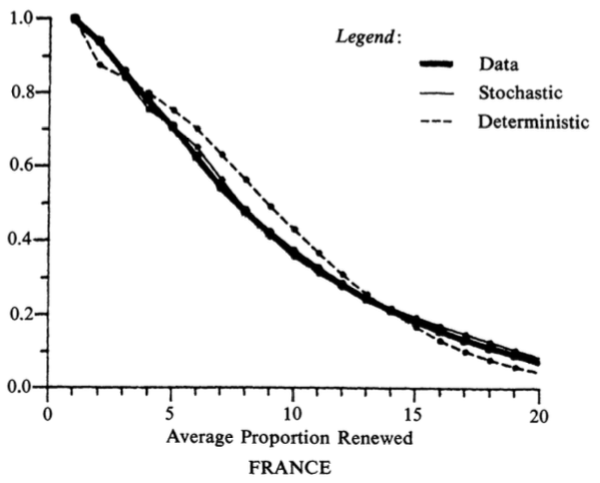
\includegraphics[scale=.34]{pakes86_f4a}
	
% }

% \frame{
% 	\frametitle{Pakes (1986)}
% 		\centering
% 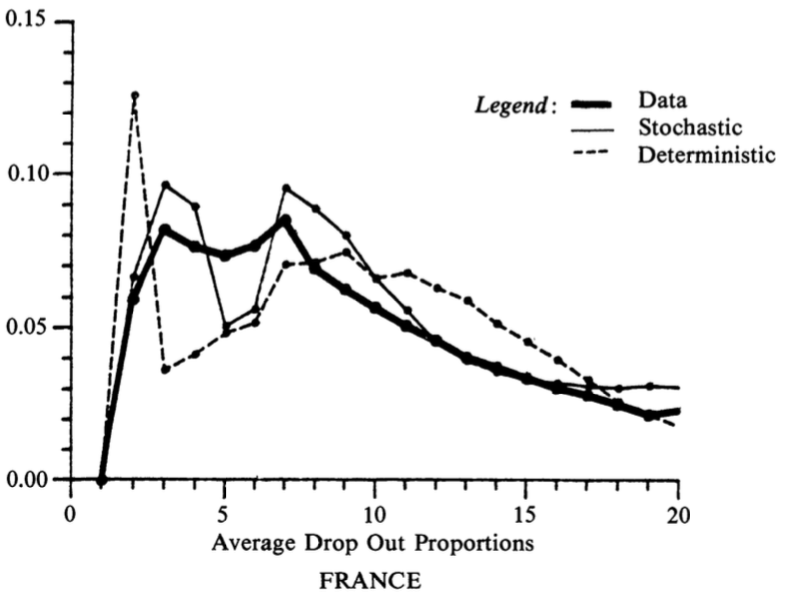
\includegraphics[scale=.34]{pakes86_f5a}
	
% }

\begin{frame}[plain]
\footnotesize
\vspace{1.1cm}
\begin{center}
\huge 
\textbf{DDC Estimation via OLS}
\end{center}
\end{frame}


% \frame{
% \frametitle{Scott (2016)}
% \framesubtitle{Evaluate biofuels policy}

% \textbf{Applied question}
% \begin{itemize}
% \item[$-$] What are the effects of biofuels policy?
% \item[$-$] US biofuels mandate: about 10\% of gasoline must come from biofuels
% (Renewable Fuels Standard)
% \end{itemize}

% \textbf{Dynamics versus Statics}
% \begin{itemize}
% \item[$-$] How to estimate long-run elasticities of crop supply?
% \item[$-$] Relevant for many agricultural and environmental policy questions.
% \item[$-$] Supply elasticities based on static models might be downwards-biased. 
% \end{itemize}

% \textbf{Contributions}
% \begin{itemize}
% \item[$-$] Develops tractable and flexible dynamic model of land  use.
% \item[$-$] Taking dynamics into account implies larger environmental impacts,
% smaller price impacts from biofuels.
% \end{itemize}

% }




% \frame{
% \frametitle{Scott (2016)}
% \framesubtitle{Evaluate biofuels policy}
% \begin{itemize}


% \medskip
% \item[$-$] Appeal of biofuels: closing the carbon cycle
% \begin{itemize}
% \item[$-$] But what is the opportunity cost of the feedstock?
% \end{itemize}

% \medskip
% \item[$-$] Biofuels mandate $\rightarrow$ a long-run increase in demand for grains
% \begin{itemize}
% \item[$-$] 35-40\% of US corn production used to for ethanol recently.
% \end{itemize}

% \medskip
% \item[$-$] Increased demand $\rightarrow$ higher food prices and/or environmentally
% destructive land use change


% \end{itemize}

% }



% \frame{
% \frametitle{Intensive vs. extensive margins}

% \begin{itemize}
% \item[$-$] Focus is on the \textbf{extensive margin} of agricultural supply, i.e. land use change.

% \bigskip
% \item[$-$] \textbf{Intensive} margin assumed to be small.

% \bigskip
% \item[$-$] Supporting evidence: Berry and Schlenker (2011), Scott (2013), Sant'Anna (2015).

% \end{itemize}

% }


% \frame{
% \frametitle{Scott (2016)}
% \framesubtitle{Methodological Contribution}
% \begin{itemize}

% \begin{itemize}
% \item[$-$] landowners may respond differently to different types of price variation
% \item[$-$] important if we want to predict response to counterfactual price variation
% that is (potentially) different than the type of price variation in the data

% \end{itemize}
% \end{itemize}
% }



\frame{
\frametitle{Scott (2016)}
\framesubtitle{Overview}
\small 

\textbf{Applied question}
\begin{itemize}\footnotesize
\item[$-$] What are the effects of biofuels policy?
\item[$-$] US biofuels mandate: $\approx$ 10\% of gasoline must come from biofuels.
\item[$-$] Supply elasticities based on static models might be downwards-biased. 
\end{itemize}

\vspace{0.3cm}

Estimate model using \textbf{linear regression}.
\begin{itemize}\footnotesize
\item[$-$] Relies on Hotz-Miller (1993) inversion.
\item[$-$] Exploits finite dependence, Altug and Miller (1998).	
\item[$-$] Can be seen as an \textbf{``Euler equation''} approach for DDC models.
\end{itemize}


}

\frame{
\frametitle{Scott (2016)}
\framesubtitle{Method}
\small 
\textbf{Key insight:}
\begin{itemize}\footnotesize
\item Realizations of agents future utility are noisy measures of agent's expectation.
\end{itemize}

\vspace{0.3cm}

\textbf{Advantages of approach:}
\begin{itemize}\footnotesize
\item[$-$] No need to specify how all state variables evolve over time. 
\end{itemize}

\vspace{0.3cm}

Can be combined with \textbf{quasi-experimental} variation:
\begin{itemize}\footnotesize
\item[$-$] Diamond, McQuade, Qian (2018): combine with diff-in-diff IV to study rent control.
\item[$-$] No need to explicitly model expectations. 
\end{itemize}

}






\frame{
\frametitle{Scott (2016)}
\framesubtitle{Model + Assumptions}
\footnotesize 
\textbf{Binary crop choice model}

A landowner's choice set: $\mathcal{A}=\left\{ crops,other\right\} $. If field $i$ is in state $x$ at time $t$, then the \emph{expected} profits to land use $j$ are:
\vspace{-0.2cm}
\[
\pi\left(a,x,\omega_{t},\nu_{it}\right)=\alpha_{0,a,x}+\alpha_{R}\cdot R_{a}\left(\omega_{t}\right)+\xi_{a,x}\left(\omega_{t}\right)+\nu_{iat}
\]
\vspace{-0.2cm}
\smallskip{}

\textbf{Notation:}
$i$: field,$a$: land use, $k$: field state, $\omega$: market state, $R$: expected returns, observable to econometrician,
$\xi$: unobservable shock to returns, $\nu$: idiosyncratic field-level shock,
$\alpha$: parameters to be estimated,


\textbf{Assumptions:}
\begin{enumerate}\footnotesize 
\item Small fields, no externalities: the distribution of the market state $\omega_{t+1}$ conditional on
$\omega_{t}$ is not affected by changing the land use in any single field.
\item Logit errors: The idiosyncratic error term $\nu_{iat}$ has a type 1 extreme value
distribution, independently and identically distributed across $i$, $a$, and $t$.
\item Landowners have rational expectations.
\end{enumerate}

}



\frame{
\frametitle{Scott (2016)}
\framesubtitle{Dynamics: Field-Level}
\vspace{-0.5cm}
\small
Landowners maximize expected discounted profits. Field states evolve according to a simple deterministic process:
\[
x_{i,t+1}=x^{+}\left(a_{it},x_{it}\right)=\begin{cases}
0 & \mbox{if }a_{it}=crops\\
\min\left\{ x_{it}+1,\bar{x}\right\}  & \mbox{if }a_{it}=other
\end{cases}
\]

\textbf{Important details:} 
\begin{itemize}\footnotesize 
\item[$-$] Like in bus-engine replacement, there is a renewal action.


\item[$-$] No explicit assumptions on the evolution of $R$ and $\xi$

\item[$-$] Estimating the process governing the evolution of the unobservable
supply shock $\xi$ is especially difficult. 
\end{itemize}

}


% \frame{
% \frametitle{Dynamics: Alternative}

% \begin{itemize}
% \item[$-$] Alternative field-level dynamics:
% \[
% k_{i,t+1}=x^{+}^{+}\left(j_{it},x_{it}\right)=\begin{cases}
% -1 & \mbox{if }j_{it}=crops,x_{it}>0\\
% \max\left(k-1,-\bar{k}\right) & \mbox{if }j_{it}=crops,x_{it}<0\\
% 1 & \mbox{if }j_{it}=other,x_{it}<0\\
% \min\left(k+1,\bar{k}\right) & \mbox{if }j_{it}=other,x_{it}>0
% \end{cases}
% \]

% \medskip
% \item[$-$] With the original $x^{+}^{+}$, $j_{it}=crops$ is a renewal action \\
% here, $\left(j_{it},j_{i,t+1}\right)=\left(crops,other\right)$ is a renewal sequence
% \end{itemize}
% }

% \frame{
% \frametitle{Scott (2016)}
% \framesubtitle{Dynamics: Value Function}
% \begin{itemize}
% \item[$-$] $\beta$: common discount factor
% \item[$-$] Value function:
% \[
% \begin{array}{l}
% V_{t}\left(k_{it},\nu_{it}\right)\equiv\\
% \quad\max_{\mathbf{j}}E\left[\sum_{s\ge t}^{\infty}\beta^{s-t}\pi\left(\mathbf{j}\left(\omega_{s},x_{is},\nu_{is}\right),x_{is},\omega_{s},\nu_{is}\right)|x_{it},\omega_{t},\nu_{it}\right]
% \end{array}
% \]
%  where $\mathbf{j}$ represents a policy function.
% \end{itemize}
% \bigskip{}



% }


\frame{
\frametitle{Scott (2016)}
\framesubtitle{Regression equation construction}

\textbf{Steps:}
\begin{enumerate}
\item Start with condition for indifferent agent\medskip
\item Introduce expectational error (\textbf{``Euler equation''} error term)\medskip
\item Forward calculation of continuation values using conditional choice
probabilities\medskip
\item Rearrange into regression equation\bigskip\medskip
\end{enumerate}
}



\frame{
\frametitle{Scott (2016)}
\framesubtitle{Dynamics: Definitions}\small
\textbf{Ex ante} value function:
\[
\bar{V}_{t}\left(x\right)\equiv\int V_{t}\left(x,\omega_t,\nu\right)dF\left(\nu\right),
\]
the value function integrated over idiosyncratic shocks $\nu$\bigskip{}.

\textbf{Choice specific} value function:
\[
v_{t}\left(a,x\right)\equiv\bar{\pi}_{t}\left(a,x\right)+\beta\cdot E_{t}\left[\bar{V}_{t+1}\left(x^{+}\left(a,x\right)\right)\right],
\]
 where $\bar{\pi}$ indicates ex ante profits (without idiosyncratic error). Conditional choice probabilities (with logit assumption):
\[
P(a|x,t)=\frac{\exp\left(v_{t}\left(a,x\right)\right)}{\sum_{j \in \mathcal{A}}\exp\left(v_{t}\left(j,x\right)\right)}
\]

}


\frame{
\frametitle{Scott (2016)}
\framesubtitle{Step 1: Indifferent agent condition (HM-inversion)}
\small
The \textbf{HM inversion} with logit errors:
\[
\ln\left(\frac{P(a|x,t)}{P(a'|x,t)}\right)=v_{t}\big(a,x\big)-v_{t}\left(a',x\right)
\]
\bigskip{}

Rewrite as relationship between current profits and continuation values:
\[
\begin{array}{l}
\bar{\pi}_{t}\left(a,x\right)-\bar{\pi}_{t}\left(a',x\right)+\ln\left(\frac{P(a|x,t)}{P(a'|x,t)}\right)=\qquad\qquad\qquad\\
\\
\qquad\qquad\beta\left(E_{t}\left[\bar{V}_{t+1}\left(x^{+}\left(a',x\right)\right)\right]-E_{t}\left[\bar{V}_{t+1}\left(x^{+}\left(a,x\right)\right)\right]\right)
\end{array}
\]

Expectation over \textbf{unobserved} state variables!

}


\frame{
\frametitle{Scott (2016)}
\framesubtitle{Step 2: Expectational errors}
\footnotesize
\textbf{Expectational error:}
\[
\varepsilon_{t}^{CV}\left(a,x\right)\equiv\beta\left(E_{t}\left[\bar{V}_{t+1}\left(x^{+}\left(a,x\right)\right)\right]-\bar{V}_{t+1}\left(x^{+}\left(a,x\right)\right)\right)
\]

Adding and subtracting realizations of the value function, the condition can be rewritten:
\[
\begin{array}{l}
\bar{\pi}_{t}\left(a,x\right)-\bar{\pi}_{t}\left(a',x\right)+\ln\left(\frac{P(a|x,t)}{P(a'|x,t)}\right)=\qquad\qquad\qquad\\
\\
\qquad\qquad\beta\left(\bar{V}_{t+1}\left(x^{+}\left(a',x\right)\right)-\bar{V}_{t+1}\left(x^{+}\left(a,x\right)\right)\right)\\
\\
\qquad\qquad+\varepsilon_{t}^{CV}\left(a',x\right)-\varepsilon_{t}^{CV}\left(a,x\right)
\end{array}
\]
The expectational error terms are mean uncorrelated with any variables
in the information set $\omega_{t}$.

\vspace{0.3cm}

$\rightarrow$ Next two slides show how continuation values can be replaced in this equation to transform the problem into a \textbf{linear} estimation equation. 
}




\frame{
\frametitle{Scott (2016)}
\framesubtitle{Step 3: Forward calculation}
\small
Use Arcidiacono and Miller's lemma to replace continuation values:
\[
\bar{V}_{t}\left(x\right)=-\ln\left(P(a^\star|x,t)\right)+v_{t}\left(a^{*},x\right)+\gamma
\]
which holds for \textbf{any} land use $a^{*}$. Recall $x^{+}\left(crops,x\right)=0$ for all $x$ (renewal action). By choosing $a^{*}=crops$, continuation values from $t+2$ onward
will cancel:

\vspace{0.3cm}

\[
\hspace*{-0.5cm}
\begin{array}{ccc}
\bar{V}_{t+1}\left(x^{+}\left(a,x\right)\right) & = &
-\ln\left(P(a^{*}|x^{+}\left(a,x\right),t+1)\right)+\bar{\pi}_{t+1}\left(a^{*},x^{+}\left(a,x\right)\right)+\beta\bar{V}_{t+2}\left(0\right)+\gamma\\
\\
\bar{V}_{t+1}\left(x^{+}\left(a',x\right)\right) & = &
-\ln\left(P(a^{*}|x^{+}\left(a',x\right),t+1)\right)+\bar{\pi}_{t+1}\left(a^{*},x^{+}\left(a',x\right)\right)+\beta\bar{V}_{t+2}\left(0\right)+\gamma
\end{array}
\]
}








\frame{
\frametitle{Scott (2016)}
\framesubtitle{Step 4: rearrange into regression equation}
\small
\vspace{-0.6cm}
\[
Y_{x,t}=\tilde{\Delta}\alpha_{0}\left(x\right)+\alpha_{R}\Delta R_{t}+\tilde{\Delta}\xi_{xt}+\Delta\varepsilon_{t}^{CV}
\]
where
\[
{\small \begin{array}{ccc}
Y_{x,t} & = & \ln\left(\frac{P(crops|x,t)}{P(other|x,t)}\right)+\beta\cdot \ln\left(\frac{P(crops|0,t+1)}{P(crops|x^{+}\left(other,x\right),t+1)}\right)\\ \\
\tilde{\Delta}\alpha_{0}\left(x\right) & = & \alpha_{0,crops,x}-\alpha_{0,other,x}\\
 &  & +\beta\left(\alpha_{0,crops,0}-\alpha_{0,crops,x^{+}\left(other,x\right)}\right)\\  \\
\Delta R_{t} & = & R_{crops,t}-R_{other,t}\\ \\
\tilde{\Delta}\xi_{t} & = & \xi_{crops,x,t}-\xi_{other,x,t}+\beta\left(\xi_{crops,0,t+1}+\xi_{crops,x^{+}\left(other,x\right),t+1}\right)\\ \\
\Delta\varepsilon_{t} & = & \varepsilon_{t}^{CV}\left(crops,x\right)-\varepsilon_{t}^{CV}\left(other,x\right)
\end{array}}
\]

Generalizes to multinomial setting and (almost) any distribution for $\nu$.

}


\frame{
\frametitle{Scott (2016)}
\framesubtitle{Identification of Payoff Parameters}\small
\vspace{-0.3cm}
\begin{itemize}\footnotesize
	\item[$-$] The regression identifies one value for each $x$:  \[
 \begin{array}{ccl}
\tilde{\Delta}\alpha_{0}\left(x\right) & = & \alpha_{0,crops,x}-\alpha_{0,other,x}\\
 &  & +\beta\left(\alpha_{0,crops,0}-\alpha_{0,crops,x^{+}\left(other,x\right)}\right)\\
\end{array}
\]


	\item[$-$] However, we have $2|x|$ values of $\alpha_{0}$ in the profit function for each $x$:
	$\alpha_{0,crops,x}$ and $\alpha_{0,other,x}$. For identification, assume that $\alpha_{0,other,x}=0$ for all $x$.

	\item[$-$] Such restrictions are often called {}``normalizations'' in the literature, but they are substantive restrictions in principle (Magnac and Thesmar, 2002).

	\item[$-$] However, more recent work (Norets and Tang, 2014; Kalouptsidi, Scott, and Souza-Rodrigues 2015)
	has considered whether these restrictions actually matter for counterfactuals.

	\item[$-$] Turns out counterfactuals in this paper (i.e., long run elasticity calculations) are identified, meaning that the above restriction is harmless.
	

\end{itemize}
}



% \frame{
% \frametitle{Identification of counterfactuals}
% \begin{itemize}\small 
% 	\item[$-$] For identification, I assume that $\alpha_{0,other,k}=0$


% \end{itemize}
% }

% \frame{
% \frametitle{Heterogeneity}

% \begin{itemize}
% \item[$-$] $z_{i}$: observable persistent field-level characteristic (counties)

% \bigskip
% \item[$-$] $\zeta_{i}$: Persistent, unobservable field-level characteristic (binary)

% \begin{itemize}
% \item[$-$] estimation idea: EM algorithm (Arcidiacono and Miller, 2011)
% \end{itemize}
% \end{itemize}
% }


% \frame{
% \frametitle{Estimation without unobservable heterogeneity}
% \begin{enumerate}
% \item[$-$] Estimate conditional choice probabilities \textcolor{white}{\textbf{for each unobservable type using EM algorithm}}

% \medskip
% \item[$-$] Construct dependent variable from CCP estimates

% \medskip
% \item[$-$] Linear regression to estimate $\tilde{\Delta}\alpha_{z,\zeta,0}\left(k\right)$
% and $\alpha_{R}$

% \medskip
% \item[$-$] Recover $\alpha_{z,\zeta,0}\left(j,k\right)$ from $\tilde{\Delta}\alpha_{z,\zeta,0}\left(k\right)$
% \end{enumerate}

% }


% \frame{
% \frametitle{Estimation with unobservable heterogeneity}
% \begin{enumerate}
% \item[$-$] Estimate conditional choice probabilities \textbf{for each unobservable type using EM algorithm}

% \medskip
% \item[$-$] Construct dependent variable from CCP estimates

% \medskip
% \item[$-$] Linear regression to estimate $\tilde{\Delta}\alpha_{z,\zeta,0}\left(k\right)$
% and $\alpha_{R}$

% \medskip
% \item[$-$] Recover $\alpha_{z,\zeta,0}\left(j,k\right)$ from $\tilde{\Delta}\alpha_{z,\zeta,0}\left(k\right)$
% \end{enumerate}

% }



% \frame{
% \frametitle{Identification of unobservable heterogeneity}

% % \begin{center}
% % \includegraphics[scale=0.65]{/Users/paul/Dropbox/land_use_change/data_backup/r1_binary_ccps}
% % \par\end{center}

% \medskip

% Formal identification papers: Hall and Zhou (2003), Kasahara and Shimotsu
% (2009) \hyperlink{UnobsHet2}{\beamergotobutton{EM details}}

% }





% \frame{
% \frametitle{Identification of unobservable heterogeneity Crop Returns}
% \begin{itemize}

% \medskip
% \item[$-$] Returns to cropland is a weighted average across crops:
% \[
% R_{crops,t,z}=\frac{\sum_{c\in\mathbf{C}}A_{cts}R_{ctz}}{\sum_{c\in\mathbf{C}}A_{cts}}
% \]
% where $A_{cts}$ is the harvested area for US state $s$.

% \medskip
% \item[$-$] $\mathbf{C}=$\{corn, soybeans, winter wheat, durum wheat, other wheat,
% barley, oats, rice, upland cotton, pima cotton\}


% \medskip
% \item[$-$] Expected returns $R_{c,t,z}$ measure the expected returns during
% \emph{planting season}:
% \[
% R_{ctz}=\left(P_{ctz}-e_{ctz}\right)\cdot YIELD_{ctz}
% \]

% \end{itemize}
% }




% \frame{
% \frametitle{Expected yields}
% \begin{itemize}
% \item[$-$] Yields based on weather data, county fixed effects, and a linear time
% trend:
% \[
% \ln\left(YIELD_{ctz}\right)=\theta_{cz}+\theta_{cw}W_{tz}+\theta_{ct}t+\varepsilon_{ctz}
% \]

% \item[$-$] For county-crops with insufficient data, I impute fixed effects based
% on a weighted average of fixed effects for nearby counties.

% \bigskip
% \item[$-$] Weather data and specification from Schlenker and Roberts (PNAS, 2009).

% \end{itemize}
% }





% \frame{
% \frametitle{Identification: first differences}

% \[
% \begin{array}{cc}
% Y_{n,t+1}-Y_{nt}= & \alpha_{R\zeta}\left(R_{n,t+1}-R_{nt}\right)\\
% \\
%  & +\tilde{\Delta}\xi_{n,t+1}-\tilde{\Delta}\xi_{n,t}\\
% \\
%  & +\tilde{\Delta}\varepsilon_{n,t+1}^{V}-\tilde{\Delta}\varepsilon_{nt}^{V}
% \end{array}
% \]

% I use the following moments for estimation:
% \[
% E\left[\left(\begin{array}{c}
% 1\\
% R_{nt}\\
% CYIELD_{nt}
% \end{array}\right)\left(\tilde{\Delta}\xi_{n,t+1}-\tilde{\Delta}\xi_{n,t}\right)\right]=0
% \]
% where $CYIELD_{nt}$ is expected caloric yield.

% }


\frame{
\frametitle{Scott (2016)}
\framesubtitle{Conclusion}
{\small
\begin{itemize}\small
	\item Fully dynamic model estimated with regression equation
	\item Euler equation approach avoids the need for a full model of state variables; data limitations show up in an error term (like static applied micro models) rather than necessarily leading to model misspecification.
	\item Can be combined with quasi-experimental techniques. 
	\item Depending on the size of the state space, not all cells in $p(.|x,t)$ might be populated. Might have to interpolate, for example, through kernel smoothing.
\end{itemize}
}
}




\frame{
\frametitle{Autocorrelated Unobservables}
\framesubtitle{Some other relevant work}
\small
Related work to take care of endogeneity issues caused by \textbf{autocorrelated} unobserved state variables:

\vspace{0.5cm}

\textbf{Berry and Compiani (2017)}: \textit{An Instrumental Variable Approach to Dynamic Models}
\begin{itemize}\small
\item Generalized instrumental variable approach (Chesher and Rosen (2015)).
\item Set identification, estimator is discrete grid search. 
\end{itemize}


\textbf{Kalouptsidi et Al. (2017)}: \textit{An Instrumental Variable Approach to Dynamic Models}
\begin{itemize}\small
\item Linear IV approach builds on Scott's Euler equations insight. 
\end{itemize}



}




\begin{frame}[plain]
\footnotesize
\vspace{1.1cm}
\begin{center}
\huge 
\textbf{Simulation Estimation}
\end{center}
\end{frame}


\frame{
	\frametitle{Pakes (1986): Patents as Options}
		\framesubtitle{Overview}
\small

\textbf{The patent literature:}

\begin{itemize}\footnotesize
	\item Intellectual property (what is the value of patents?)
	\item Measuring the causes, effects and distribution of benefits from innovation (often uses patent counts and author linkages).
	\item Important input to inform optimal length of patents. 
\end{itemize}

\textbf{Main idea}
\begin{itemize}\footnotesize
	\item In many countries, patent holders required to pay renewal fee to keep patents in force.
	\item More than 90\% of patent holders let patents expire before the limit on patent lives.
	\item Use patent renewal decisions and costs of renewal to infer the distribution of patent values. Patents as options.
\end{itemize}


\textbf{Methodological contributions}
\begin{itemize}\footnotesize
	\item Simulation estimator, serially correlated unobserved state variable (relaxes iid, conditional logit assumptions)
\end{itemize}
}


\frame{
	\frametitle{Pakes (1986): Patents as Options}
	\centering
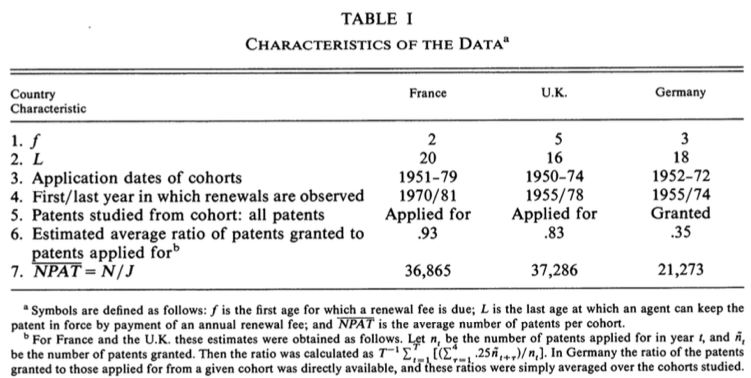
\includegraphics[scale=.45]{pakes86_t1}
	
}


\frame{
	\frametitle{Pakes (1986): Patents as Options}
		\centering
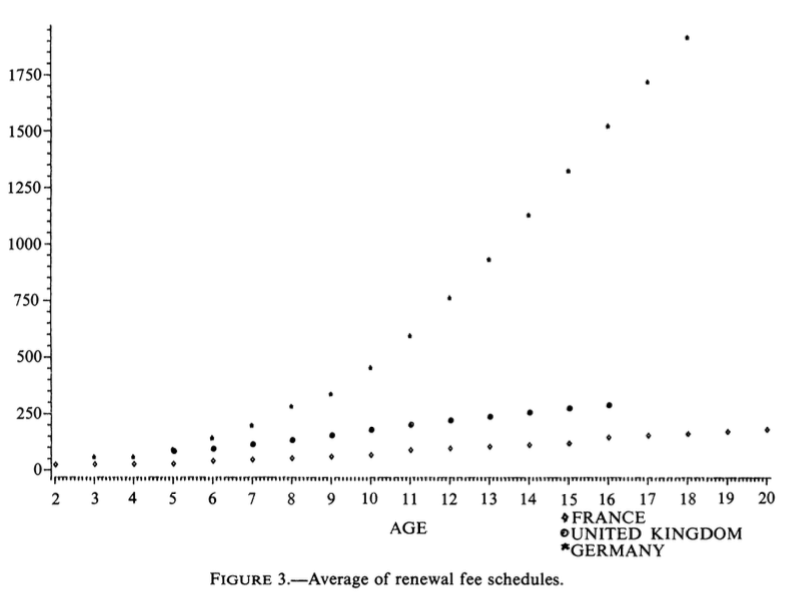
\includegraphics[scale=.35]{pakes86_f3}
	
}


\frame{
	\frametitle{Pakes (1986): Patents as Options}
	\framesubtitle{Model Details}\small
% \textbf{Main idea:}

\begin{itemize}
\footnotesize
	\item This is, again, an optimal stopping problem!

	\item First year returns from patent protection are $r_1$. (May be only small part of total returns to the patented idea).
	
	\item Returns in future years $r_2,r_3,...$ are random.
	\item Cost of renewing each year $c_1,c_2,...$
	\item \underline{2 period intuition}:
		\begin{itemize}\footnotesize
			\item 2nd period: renew if $r_2>c_2$, so obtain $\max \{r_2-c_2,0\}$
			\item First period (if renew):
				
				\[ r_1 -c_1 + \beta \int \max \{ r_2-c_2,0 \} P(dr_2 \vert r_1) \]
			
			\item $P$ stochastically increasing in $r_1$.
			\item There is a cutoff $\bar{r}_1 < c_1 $ s.t. if $r< \bar{r}_1$, patent is not renewed.
			\item Second period cutoff is simply $\bar{r}_2 = c_2$.
		\end{itemize}
\end{itemize}
}


\frame{
	\frametitle{Pakes (1986): Patents as Options} 
	\framesubtitle{Model Details}
\footnotesize
% \textbf{Primitives, parameterized by $\theta$}

\vspace{0.3cm}

$\Omega_a:$ history of returns up to age, $\{r_1,...,r_a\}$. The expectation is over $r_{a+1}|\Omega_a$. The sequence of conditional distributions $F(a_{t+1}|\Omega_a), a = 1,2,...$ is an important component of the model. Pakes' assumption: 

\vspace{-0.4cm}

\begin{align*}
r _ { a + 1 } = \left\{ \begin{array} { l l } { 0 } & { \text { with prob. } \exp \left( - \theta r _ { a } \right) } \\ { \max \left( \delta r _ { a } , z \right) } & { \text { with prob. } 1 - \exp \left( - \theta r _ { a } \right) } \end{array} \right.
\end{align*}

where density of $z$ is $q _ { a }(z) = \frac { 1 } { \sigma _ { a } } \exp \left[ - ( \gamma + z ) / \sigma _ { a } \right]$ and $
\sigma _ { a } = \phi ^ { a - 1 } \sigma , a = 1 , \dots , L - 1$.

\vspace{0.4cm}

Sequence of renewal fees $\{ c_a \}$, increasing in age. Gives rise to value function:

\[V(r,a)=\begin{cases}
\begin{array}{c}
\max\{0,r-c_{a}+\beta E\left[V(r',a+1)\vert r,a\right]\}\\
\max\{0,r-c_{A}\}
\end{array} & \begin{array}{c}
\text{if }a<A\\
\text{if }a=A
\end{array}\end{cases}
\]	

}




% \frame{
% 	\frametitle{Pakes (1986): Patents as Options: Model Details}
% \small



% }







\frame{
	\frametitle{Pakes (1986): Patents as Options} 
	\framesubtitle{Model Details}
\small
\textbf{A note on the nature of this problem:} Since the maximal age is finite this is a finite horizon (non-stationary) dynamic optimization problem. Most dynamic problems fall into two camps (i) infinite horizon stationary problems and finite horizon, non-stationary problems. Stationarity just means that the value functions and optimal decision rules are \textit{time-invariant} functions of the state variables. 

\vspace{0.6cm}

\textbf{Solution is a cut-off strategy:}
\begin{itemize}\footnotesize
	\item Note that agent renews if $r+\beta E[V(r',a+1) \vert r,a] > c_a $. Since this is strictly increasing in $r$ at each $a$, there exists a unique cutoff $\bar{r}_a < c_a$ s.t. patent is renewed iff $r>\bar{r}_a.$

	\item $\bar{r}_a < \bar{r}_{a+1} < ... < \bar{r}_A = c_A$ (The fact that renewal fees are increasing in age, while the option value is decreasing,
implies that cutoffs are increasing in age.). Solved for starting in the last period.

\end{itemize}
}

\frame{
	\frametitle{Pakes (1986): Patents as Options}
	\framesubtitle{Simulation Estimator}
\small

\textbf{Outer loop:} is concerned with evaluating likelihood that arises from a complicated integral:
\begin{itemize}
	\footnotesize
	\item Maximize log-likelihood: $\log \mathcal{L}(\theta) = n^{-1} \sum_a s(a) \log \pi_a (\theta)$.
		\begin{itemize}
			\footnotesize
			\item $n$ is \# of patents in cohort
			\item $s_a$ is the fraction of the original sample dropping out at age $a$ (or surviving until terminal year if $a=A$.
			\item $\pi_a (\theta)$ is probability of dropping out at age $a$.
		\end{itemize}
	\item If $F(r,a;\theta)$ be the distribution of patent values at age $a$ we have $\pi_a(\theta) = F(\bar{r}_a,a;\theta) - F(\bar{r}_{a-1}, a-1; \theta)$
	
	\item Issue: family $\{ F(\cdot,\cdot;\theta) \} $ is complicated (not analytic).
\end{itemize}

\vspace{0.4cm}

\textbf{Inner loop:} solve the agent's problem.

}





\frame{
	\frametitle{Pakes (1986): Patents as Options}
	\framesubtitle{Simulation Estimator}
\small
\vspace{-0.2cm}
\textbf{Inner loop procedure}: backwards induction.

\begin{itemize}\footnotesize
\item At $L$ there is no more continuation value, return is $r_L$.
\item At $L-1$ solve for a grid of interest rates...interpolate (expectations over returns depend on parameter guess).
\item ...
\item This procedure gives the cut-offs needed for the outer loop. 
\end{itemize}
\vspace{-0.2cm}
\textbf{Outer loop procedure}: simulation estimator.
\begin{itemize}\footnotesize
	\item Start with a draw $r_1 \sim f(r,1;\theta)$.
	\item Let $\bar{r}_t$ be cut-off from value functions, at iteration $t<A$:
		\begin{itemize}
			\footnotesize
			\item If $r_t \geq \bar{r}_t (\theta)$, take a draw from $r_{t+1} \sim P(\cdot \vert t,r_t;\theta)$.
				\begin{itemize}
					\footnotesize
					\item i.e., stayed in at $t$
				\end{itemize}
			\item if $r_t < \bar{r}_t (\theta)$, up counter for $\hat{\pi}_t(\theta)$ by one.
				\begin{itemize}
					\footnotesize
					\item i.e., dropped out
				\end{itemize}
		\end{itemize}
	\item Use $\hat{\pi}_t(\theta) / (NSIM)$ as estimate of probability of dropping out at age $a$ (conditional on making it to that point) to compute likelihood.
\end{itemize}

}

\frame{
	\frametitle{Pakes (1986)}
		\centering
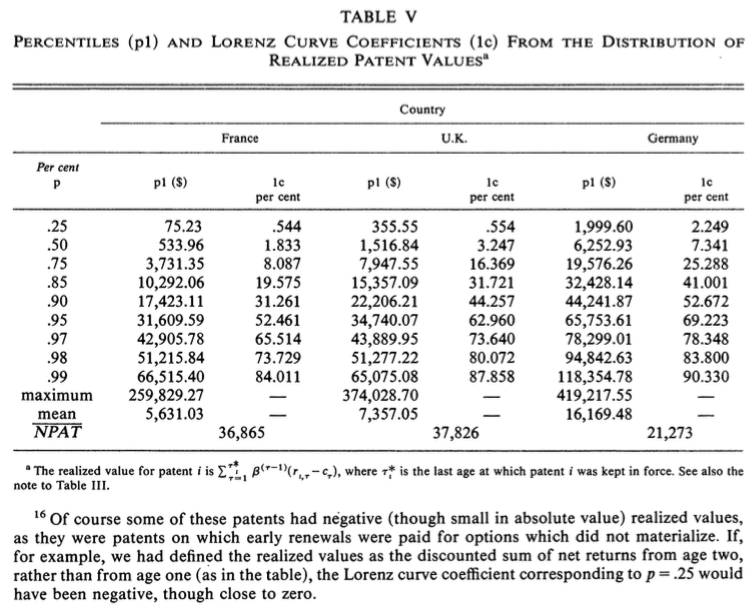
\includegraphics[scale=.35]{pakes86_t5}
	
}


\frame{
	\frametitle{Pakes (1986)}
		\centering
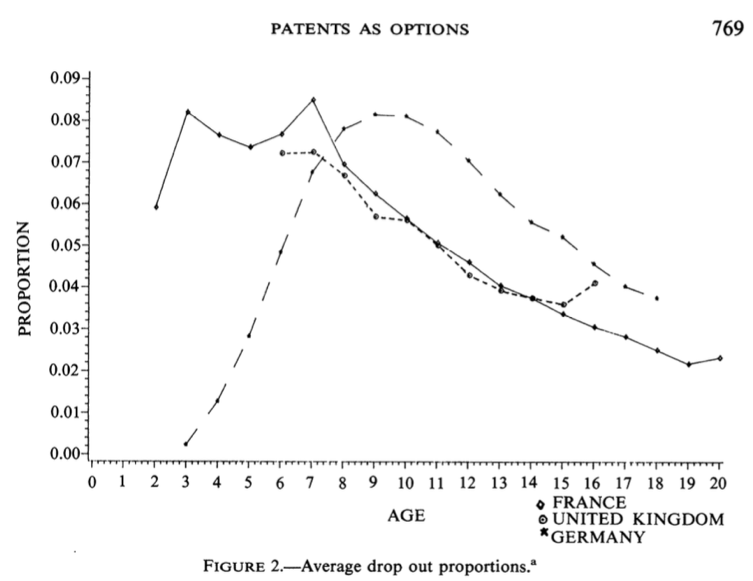
\includegraphics[scale=.35]{pakes86_f2}
	
}



\frame{
	\frametitle{Pakes (1986): Patents as Options}
		\framesubtitle{Conclusion}
\small

\begin{l_itemize}
\item Important question, how to value patents absent transaction data that would pin down their value directly.  
\item Paper was one of the first using simulation for estimation in economics (Lerman and Manski, 1981).
\item One limitation of the paper is that renewing a patent is cheap, but the aggregate value of patents is really driven by the upper tail of values (most patents turn out to be worth zero).
\item This upper tail is identified only by the strong functional form
assumption - but not obvious how else you might pin it down.
\item Non-parametric identification for these types of models not fully worked out. 
\end{l_itemize}	



}


\begin{frame}[plain]
\footnotesize
\vspace{1.1cm}
\begin{center}
\huge 
\textbf{Dynamic Demand}
\end{center}
\end{frame}



\begin{frame}{Dynamic Demand}
\framesubtitle{Two Examples}
\scriptsize
\vspace{-0.2cm}
We have covered static models of demand, such as BLP (1995). We have also looked at single agent models of dynamic behavior such as Rust (1987). What if we could put those two together? Why?

\textbf{Example: Durable Goods}
\vspace{-0.1cm}
\begin{itemize}\scriptsize
\item[$-$] We are often interested in the case where a firms' products compete not only against products of other firms, but also with their own products over time. This is a feature of many durables.
\item[$-$] In high-tech products, we have `S'-shaped penetration curve. At some point prices are cut and the sales go down rather than up. Why?
\end{itemize}
\vspace{-0.2cm}
\textbf{Example: Storable Goods}
\vspace{-0.1cm}
\begin{itemize}\scriptsize
\item[$-$] Laundry detergent goes on discount: $\approx$ 1 week in every 4-5. A large fraction of overall quantity is sold during these discount weeks.
\item[$-$] This would imply highly elastic demand. (1) Laundry detergent business must be extremely competitive. (2) There would be a substantial response to a \textbf{permanent} price change. Seems unlikely that (1) and (2) are true.
\end{itemize}

We already discussed \textbf{Hendel and Nevo (2006)} and will now look at \textbf{Gowrisankaran and Rysman (2012)}. Both are unusual for modern IO in that they are pure measurement exercises; no counterfactuals. They illustrate nicely how we would obtain biased demand estimates without considering dynamics. 

\end{frame}



\begin{frame}{Gowrisankaran and Rysman (2012)}
\begin{figure}[htbp]
\begin{center}
\includegraphics[width=3.8in]{resources/gandr1.pdf}
\label{gandr1}
\end{center}
\end{figure}
\end{frame}


\begin{frame}{Gowrisankaran and Rysman (2012)}
\begin{figure}[htbp]
\begin{center}
\includegraphics[width=3.8in]{resources/gandr2.pdf}
\label{gandr2}
\end{center}
\end{figure}
\end{frame}

%\begin{frame}{Dynamic Demand}
%\begin{figure}[htbp]
%\begin{center}
%\includegraphics[width=3.8in]{resources/conlon1.pdf}
%\label{conlon1}
%\end{center}
%\end{figure}
%\end{frame}
%
%\begin{frame}{Dynamic Demand}
%\begin{figure}[htbp]
%\begin{center}
%\includegraphics[width=3.8in]{resources/conlon2.pdf}
%\label{conlon1}
%\end{center}
%\end{figure}
%\end{frame}


\begin{frame}{Dynamic Demand}
\framesubtitle{Some Observations about Consumer Electronics}
\begin{l_itemize}\footnotesize
\item[$-$] Today a 55" 4K LCD TV (8M pixels) is \$330. In 2006, you could buy a 32" 720P (< 1M pixels) TV for $>\$10,000$.
% \item[$-$] In December 2011 TV prices fell $17\%$ on an annual basis and computer equipment fell $14\%$.
%\item[$-$] Conlon 2016 reports a 22\% annualized price decline in LCD TV's from 2006-2009.
% \item[$-$] From August 2005 to August 2015 prices declined by 87.2\%.
\item[$-$] Over time consumers buy better cameras, smart phones, or larger TV's
\item[$-$] The BLS tries to do \textit{chaining} and \textit{quality adjustments} but in high-tech products this can be very difficult.
\item[$-$] This has a potentially large impact on price indices (a small bias in the CPI can be billions of dollars in SSA/Medicare payments).
% \item[$-$] Depending on the time period we might find that demand slopes upwards (lower prices lead to lower sales)
\end{l_itemize}
\end{frame}

\begin{frame}{Gowrisankaran and Rysman (2012)}
\framesubtitle{Setup}
\small
Each consumer type is subscripted by $i$, and chooses a product $j$ in period $t$ to maximize utility:
\begin{eqnarray*}
u_{ijt} &=&   \underbrace{\alpha_i^x x_{jt} +  \xi_{jt}}_{f_{jt}} - \alpha_{i}^p p_{jt} + \varepsilon_{ijt} \\
 u_{i0t} &=&  f_{i0t} + \varepsilon_{i0t} 
\end{eqnarray*}
In the static model we have $f_{i0t} = 0$ for every $i,t$.\\
\begin{itemize}\footnotesize
\item[$-$] Consumers are heterogeneous. Dynamic replacements will lead to a law of motion $w_{i,t+1} =h(w_{i,t},s_{ijt})$.
\item[$-$] Where does the bias in the static model arise from? Correlation between $f_{i0t}$ and prices.
\end{itemize}
\vspace{0.2cm}
We can think about dynamic models as having time varying utility for the outside option $f_{i0t}$. Consumers are \textbf{forward looking} regarding durables they will own in the future.

\end{frame}

\begin{frame}
\frametitle{Gowrisankaran and Rysman (2012)}
\framesubtitle{Outside Good}\small
Goal is to endogenize the utility of the outside option $f_{i0t}$:
\begin{itemize}\footnotesize
\item[$-$] Previous choice(s): $f_{ij,t-1}$.
\item[$-$] Consumer's best option from tomorrow's market
\end{itemize}
\vspace{-0.1cm}
\textbf{Ad-Hoc approach:}
\begin{itemize}\footnotesize
\item[$-$]  Just proxy with a time trend (Lou Prentice Ying 2012), (Eizenberg 2011) etc.  That is $f_{i0t} = \gamma_{0i} + \gamma_{1i} t + \gamma_{2i} t^2 + \ldots$
\item[$-$] Can still yield the correct elasticity.
\item[$-$] Not structural. When is this a problem?
\end{itemize}

\textbf{Here:}
\vspace{-0.4cm}
\begin{multline*}
V_i(f_{i0t},\varepsilon_{i t}, \Omega_t) = \max \{ f_{i0t} + \beta\cdot E_{\Omega}[ E_{\varepsilon} V_i (f_{i0t}, \varepsilon_{it}, \Omega_{t+1}) |\Omega_{t} ] ,\\
\max_j f_{ijt}  -\alpha_i p_{jt} + \beta\cdot E_{\Omega}[ E_{\varepsilon} V_i (f_{ijt}, \varepsilon_{it}, \Omega_{t+1}) |\Omega_{t} ]  \}
\end{multline*}

where $\Omega$ is state implied by product selection and prices in the market.

\end{frame}

% \begin{frame}
% \frametitle{Gowrisankaran and Rysman (2012)}
% \framesubtitle{Assumptions}\small
% For the dynamic model we place restrictions on $f_{i0t}$:
% \begin{itemize}\footnotesize
% \item[$-$] Rational Expectations: $E[f_{i0,t+1} | \Omega_t ] =f_{i0,t+1}$.
% \item[$-$] Law of motion for consumer types:  
% \item[$-$] We can formally write down a dynamic programming problem that consumers solve:
% \end{itemize}

% \end{frame}

\begin{frame}
\frametitle{Gowrisankaran and Rysman (2012)}
\framesubtitle{Replacement Problem}\small
This Bellman defines a \textbf{Replacement Problem}.
\begin{l_itemize}\footnotesize
\item[$-$] You own a single durable good with the option to \textit{upgrade} in each period.
\item[$-$] When you upgrade you throw away the old durable and \underline{get nothing in exchange}.
\item[$-$] After a purchase $j$  you receive flow utility $f_{i0t+1} = f_{ijt}$ each period if you don't make a new purchase.
\item[$-$] We could add in depreciation if we wanted to.
\item[$-$] Other studies of durables have focused on \textit{Secondary Markets} or \textit{Perfect Rental Markets}.
\item[$-$] \textit{Resale:} Important for cars, less relevant for high-tech.
\end{l_itemize}
\end{frame}



\begin{frame}
\frametitle{Gowrisankaran and Rysman (2012)}
\framesubtitle{Inclusive Value}\small
It is helpful to use \textbf{Rust's Trick} and write: $EV_i(f_{i0t},\Omega_t)= \int V_i(f_{i0t},\varepsilon_{it},  \Omega_t)f(\varepsilon)$. 
\begin{multline*}
V_i(f_{i0t},\varepsilon_{i t}, \Omega_t) = \max \{ f_{i0t} + \beta E_{\Omega}[ EV_i (f_{i0t}, \Omega_{t+1}) |\Omega_{t} ] + \varepsilon_{i0t},\\
\\max_j f_{ijt}  -\alpha_i p_{jt} + \beta E_{\Omega}[ E V_i (f_{ijt}, \Omega_{t+1}) |\Omega_{t}] + \varepsilon_{ijt}  \}
\end{multline*}
We can write the \textbf{ex-ante} expected utility of purchasing in period $t$ without having to condition on which good you purchase:
\begin{multline*} 
\delta_{i}(\Omega_t) = E_{\varepsilon} [ \max_j f_{ijt}  -\alpha_i p_{jt} + \beta E_{\Omega}[ E V_i (f_{ijt}, \Omega_{t+1}) |\Omega_{t}] + \varepsilon_{ijt}]=  \\ \log \left( \sum_j \exp[ f_{ijt}  -\alpha_i p_{jt} + \beta E_{\Omega}[ E V_i (f_{ijt}, \Omega_{t+1}) |\Omega_{t}] ]  \right)
\end{multline*}
\end{frame}

\begin{frame}
\frametitle{Gowrisankaran and Rysman (2012)}
\framesubtitle{Inclusive Value Sufficiency}\small
\vspace{-0.8cm}
\begin{eqnarray*}
\small EV_i(f_{i0}, \Omega) = \log\left( \exp[ f_{i0} + \beta E_{\Omega'}[ EV_i (f_{i0}, \Omega') |\Omega]] + \exp(\delta_i(\Omega))  \right) + \eta
\end{eqnarray*}
\footnotesize 
where $\eta = 0.577215665$ \textit{(Euler's Constant).}\\


\vspace{0.2cm}

The fact that the expected value function depends recursively on itself and $\delta_{i}(\Omega_t)$ (Inclusive Value) leads to the following assumption:
\begin{block}{\small Inclusive Value Sufficiency}\footnotesize
If $\delta_i(\Omega) = \delta_i(\tilde{\Omega})$ then $g(\delta_i(\Omega') | \Omega)= g(\delta_i(\tilde{\Omega'}) | \tilde{\Omega})$ for all $\Omega,\tilde{\Omega}$.
\end{block}
\begin{itemize}\footnotesize
\item[$-$] The idea is that $\delta$ tells me everything about the future evolution of the states
\item[$-$] More restrictive than it looks.  Is $\delta$ low because quality is low or because prices are high? Is this the result of a dynamic pricing equilibrium?
\item[$-$] Similar assumption made to keep games with many firms tractable. We will learn about this later. 
\end{itemize}
\end{frame}

\begin{frame}
\frametitle{Gowrisankaran and Rysman (2012)}
\framesubtitle{Inclusive Value Sufficiency and Rational Expectations}\footnotesize
\vspace{-0.3cm}
Under \textbf{IVS} the problem reduces to:
\begin{eqnarray*}
EV_i(f_{i0}, \delta_i) &=& \log\left[ \exp( f_{i0} + \beta E_{\Omega'}[ EV_i (f_{i0},\delta_i') |\delta_i] )+ \exp(\delta_i)  \right]\\
\delta_{i} &=& \log \left( \sum_j \exp[ f_{ijt}  -\alpha_i p_{jt} + \beta E_{\delta'}[ E V_i (f_{ijt}, \delta_i') |\delta_i ]  \right)
\end{eqnarray*}
The idea is that the inclusive value $\delta_{it}$ IS the state space, along with his current holding of the durable $f_{i0t}$. How to deal with \textbf{expectations}? 
\begin{eqnarray*}
E_{\delta'}[ E V_i (f_{ijt},\delta_i') |\delta_i ]
\end{eqnarray*}
We need to take a stand on $g_i(\delta_i' | \delta_i)$ the anticipated law of motion for $\delta_i$.  G\&R assume it follows an $AR(1)$ process.
\begin{eqnarray*}
\delta_{it+1} = \gamma_0 + \gamma_1 \delta_{it} + \nu_{it} \mbox{ with } \nu_{it} \sim N(0,\sigma_{\nu}^2)
\end{eqnarray*}
If we see $\delta_{it}$ we could just run the $AR(1)$ regression to get consumer belief's $\hat{\gamma}$
\end{frame}



\begin{frame}
\frametitle{Gowrisankaran and Rysman (2012)}
\framesubtitle{Rational Expectations-Interpolation}\small
How to compute \textbf{complicated expectations}?
\begin{eqnarray*}
E_{\delta'}[ E V_i (f_{ijt}, \delta_i') |\delta_i ,\gamma]= \int EV_i(f_{ijt},\delta_{i}') g(\delta' | \delta,\gamma)
\end{eqnarray*}
\vspace{-0.5cm}
\begin{itemize}\footnotesize
\item We need to integrate $EV(f_{ijt},\delta_i)$ (a function) over a normal density.
\item But we don't observe $EV(f_{ijt},\delta_i)$ everywhere, only on the grid points of our state space.
% \item We can fit a linear function, cubic spline, etc. over $\delta_i$ to $EV_i$ at each value of $f_{ijt}$ on our grid.
\item  We need to \textit{interpolate} $\widehat{EV}_i(\delta_i^s)$ (Linear, Cubic Spline, etc.)
\item We might as well interpolate the function at the \textit{Gauss-Hermite} quadrature nodes and weights, re-centered at $\gamma_0 + \gamma_1 \delta$ in order to reduce the number of places we interpolate $\widehat{EV_i}$.
\item Tishara will discuss \textbf{quadrature methods} in recitation (?).
\end{itemize}
\end{frame}

% \begin{frame}
% \frametitle{Rational Expectations-Alternative}
% There is an alternative method that is likely to be less accurate
% \begin{eqnarray*}
% E_{\delta'}[ E V_i (f_{ijt}, \delta_i') |\delta_i, \gamma ]= \int EV_i(f_{ijt},\delta_{i}') g(\delta' | \delta, \gamma)
% \end{eqnarray*}
% \begin{enumerate}
% \item[$-$] We need to integrate $EV(f_{ijt},\delta_i)$ (a function) over a normal density but we only see it at the grid points of our state space.
% \item[$-$] We could \alert{discretize $g(\delta' | \delta,\gamma)$} so that it is a valid markov transition probability matrix (TPM) evaluated only at the grid points.
% \item[$-$] Now computing the expectation is just matrix multiplication.
% \end{enumerate}
% I am a bit nervous about whether two discrete approximations will get the continuous integral correct.
% \end{frame}

\begin{frame}{The Estimation Problem}
\framesubtitle{Overview}
\small
We need to solve $\forall i, t $:
\begin{eqnarray*}
S_{jt} &=& \sum_i w_i s_{ijt}(f_{i0t},\delta_{it})\\
f_{ijt} &=& \overline{\alpha} x_{jt} + \xi_{jt} + \sum_l \sigma_l x_{jl} \nu_{il} \\
s_{ijt}(f_{i0t},\delta_{it}) &=& \frac{\exp[f_{ijt} - \alpha_i p_{jt} + \beta E_{\Omega'}[ EV_i (f_{ijt}, \delta_i') |\delta_i] }{\exp [EV_i(f_{i0t},\delta_{it}) ]}\\
EV_i(f_{i0}, \delta_i) &=& \log\left[ \exp( f_{i0} + \beta E_{\Omega'}[ EV_i (f_{i0}, \delta_i') |\delta_i] )+ \exp(\delta_i)  \right]\\
\delta_{i}(EV_i) &=& \log \left( \sum_j \exp[ f_{ijt}  -\alpha_i p_{jt} + \beta E_{\delta'}[ E V_i (f_{ijt}, \delta_i') |\delta_i ]  \right)\\
E[\delta_{it+1} | \delta_{it}] &=& \gamma_0 + \gamma_1 \delta_{it}\\
% w_{i,t+1} &=&h(w_{i,t},s_{ijt})\\
\end{eqnarray*}
\end{frame}


\begin{frame}{Estimation}
\framesubtitle{Algorithm}

Like BLP we guess the nonlinear parameters of the model $\theta$
\begin{enumerate}
\item \textbf{(Inner Loop)} Solve for $EV_i$ by iteratively computing $\delta$, and
running the regression for each $i$ and spline/interpolating to compute $E[EV_i]$.
\item \textbf{(Middle Loop)} G\&R use a modified version of the BLP contraction mapping. We need to make sure to update the $w_{it}$ via $h(.)$. (This is a TPM that tells maps
the transition probabilities of type i holding $f_{i,0,t}$ to $f_{i,0,t+1}$).
\item \textbf{(Outer Loop)} Once we’ve solved this whole system of equations, we use $\xi$ to form moments just
like BLP and do GMM. 
\end{enumerate}
\end{frame}


\begin{frame}{Gowrisankaran and Rysman (2012)}
\framesubtitle{COLI Index}
\begin{figure}[htbp]
\begin{center}
\includegraphics[width=3.7in]{resources/gandr3.pdf}
\label{gandr3}
\end{center}
\end{figure}
\end{frame}


\begin{frame}{Gowrisankaran and Rysman (2012)}
\framesubtitle{Conclusion}

\textbf{Elasticity measurement:}
\begin{itemize}\footnotesize 
\item \textit{Temporary price change, single camcorder:} long run and short run elasticity are close, camcorders are close substitute.
\item \textit{Temporary price change, all camcorders:} Long run elasticity is smaller than short run elasticity. 
\item \textit{Permanent price change:} long run elasticity is larger. 
\end{itemize}

\textbf{The value of new goods:}
\begin{itemize}\footnotesize 
\item COLI: Income (tax) that would make household indifferent between buying today and some later period. 	
\item G+R: People who buy later, value goods less. COLI is overstated if we interpret this as an increase in quality. 
\end{itemize}

\textbf{Other comments:}
\begin{itemize}\footnotesize 
\item No panel data, not clear what people are upgrading from.
\item No supply side, but many interesting exercises without counterfactuals.
\end{itemize}	

\end{frame}


% \begin{frame}{G\&R Parameters}
% \begin{figure}[htbp]
% \begin{center}
% \includegraphics[width=3in]{resources/gandrtable1.pdf}
% \label{conlon1}
% \end{center}
% \end{figure}
% \end{frame}

% \begin{frame}{G\&R Robustness}
% \begin{figure}[htbp]
% \begin{center}
% \includegraphics[width=3.8in]{resources/gandrtable2.pdf}
% \label{conlon1}
% \end{center}
% \end{figure}
% \end{frame}



% \begin{frame}{Perfect Foresight}
% \begin{itemize}
% \item[$-$] Contrary to the static model, price coefficient is negative (as one would expect).
% \item[$-$] Coefficients on many product characteristics are intuitively appealing.
% \item[$-$] Allowing for repeated purchases generates more ``sensible'' results.
% \item[$-$] ``Better results'' from a dynamic model may be due to the fact that people wait to purchase because of the expectations of price declines and not directly because of high prices.
% \item[$-$] Unlike the static model, in dynamic setup the explanation of waiting does not conflict with consumers buying relatively high-priced products.
% \item[$-$] A variety of robustness measures show that the major simplifying assumptions about the dynamics in the model are broadly consistent with the data.
% \end{itemize}
% \end{frame}

% \begin{frame}{Perfect Foresight}
% G\&R Report similar elasticities in the perfect foresight case. We make the following simplification
% \begin{eqnarray*}
% E_{\Omega'}[ EV_i (f_{i0}, \delta_{i,t+1}) |\delta_{i,t}] )] = EV_i (f_{i0}, \delta_{i,t+1})
% \end{eqnarray*}
% This saves us a lot of headaches:
% \begin{itemize}
% \item[$-$] No more integration/interpolation
% \item[$-$] We can solve the problem on the grid!
% \item[$-$] No more belief regressions
% \end{itemize}
% \end{frame}


% \begin{frame}{Endogeneity and Instruments}
% \begin{itemize}
% \item[$-$] Dynamics mean we  \alert{lean harder on the assumption of exogenous product characteristics} 
% \item[$-$] In one period we can take characteristics as given, but in many periods this becomes less palatable (Do cameras exogenously improve over time?).
% \item[$-$] Endogeneity: price is endogenous while other product characteristics are not, i.e. $x_{jt}$. (Size,Resolution, etc.)
% \item[$-$] Price is chosen by the firms possibly after observing $\xi_{jt}$ and, hence, is endogenous.
% \item[$-$] Instruments: use variables that affect the price-cost margin, e.g. measures of how crowded a product is in characteristics space, which effects price-cost margin and the substitutability across products.
% \begin{enumerate}
% \item[$-$]  all of the product characteristics in x;
% \item[$-$] mean product characteristics for a given firm;
% \item[$-$] mean product characteristics for all firms;
% \item[$-$] the count of products offered by the firm and by all firms.
% \item[$-$] changes in costs over time?
% \end{enumerate}
% \end{itemize}
% \end{frame}







\begin{frame}[plain]
\footnotesize

\vspace{1.1cm}
\begin{center}
\huge 
\textbf{Demand for Storable Goods}
\end{center}
\end{frame}

\begin{frame}{Demand for Storable Goods}
\vspace{-0.6cm}
\textbf{References:}
\begin{itemize}
    \footnotesize
\item[$-$] Pesendorfer (2002), Erdem, et al. (2003), Hendel and Nevo (2006).
\end{itemize}    

\textbf{Observation:}
\begin{itemize}
\footnotesize
\item[$-$] When a supermarket cuts the price of laundry detergent for a week there is a large increase in sales. This leads us to conclude consumers are extremely elastic with respect to price
\item[$-$] When a supermarket makes a permanent price cut to laundry detergent, there is little sales impact in the long run. Now consumers look highly inelastic with respect to price
\end{itemize}

\textbf{Purchasing vs. consumption elasticity}
\begin{itemize}
\footnotesize
\item[$-$] In the short-run, store-level demand elasticity reflect stockpiling behavior.
\item[$-$] In the long-run, store-level demand elasticity reflects consumption decisions.
\end{itemize}
\footnotesize

\vspace{0.1cm}
$\rightarrow$ Ignoring stockpiling and forward-looking behavior can lead to \textbf{biased own
and cross price elasticities}.

\end{frame}




\begin{frame}{Demand for Storable Goods}
\textbf{Price discrimination theory of sales:}
\begin{itemize}
\footnotesize
\item[$-$] If consumers differ in the storage costs (or credit constraints) firms have an incentive to price
discriminate. Ketchup pricing example (Pesendorfer 2002):
\end{itemize} 
\vspace{-7.0cm}   
\begin{center}
\hbox{
\hspace{-2.0cm}
\includegraphics[scale=.70]{resources/pesendorfer2002.pdf}
}
\end{center}
\end{frame}


\begin{frame}{Hendel and Nevo (2006)}
\framesubtitle{A Note on the Data}
\begin{itemize}
\footnotesize
\item[$-$] Dominick's, 9 Supermarkets in Chicago.
\item[$-$] Three years of data (1991-1993), store level and household panel. 
\item[$-$] \textbf{Store level:} For each product in each store-week observe average price, average quantity, promotions.
\item[$-$] \textbf{Household level:} Sample of households, supermarket visits, total expenditure during each visit, detailed purchase information in 24 product categories.
\item These days: \textit{Nielsen Scanner Data}, available through the \textit{Booth Kilts Center}. 
\end{itemize}
\end{frame}


\begin{frame}{Hendel and Nevo (2006)}
\framesubtitle{Reduced Form Companion Paper}
\small
\textbf{Results:}
\begin{itemize}\footnotesize
\item[$-$] Aggregate demand increases as a function of duration from previous sale, and this
effect differs between sale and non-sale periods. 
\item[$-$] Fraction of purchases on sale is higher in one market (the market that on average has larger houses), and if there is a dog in the house. Both
of these measures could potentially be correlated with lower storage costs. 
\item[$-$] When buying on sale, households tend to buy more quantity (by buying either more units or larger sizes), buy
earlier, and postpone their next purchase.
\item[$-$]  Inventory constructed under the assumption of fixed consumption over time is negatively correlated with quantity purchased and the probability of purchase. 
\item[$-$] The patterns of sales across different product categories are consistent with the variation in storage costs across these products. 
\end{itemize}
\end{frame}


% \begin{frame}{Hendel and Nevo (2006)}
% \framesubtitle{Consumers have Inventories}
% \begin{itemize}
% \footnotesize
% \item[$-$] Hendel and Nevo suggest that consumers respond by temporary price  reductions by stockpiling inventories.
% \item[$-$] Consumers spend down their inventories during periods of high prices
% \item[$-$] Consumers have variable storage costs and price sensitivities.
% \item[$-$] This has implications for inter temporal price discrimination and retail high-low pricing strategies.
% \end{itemize}
% \end{frame}




\begin{frame}{Hendel and Nevo (2006)}
\framesubtitle{Data and Model Basics}
\begin{itemize} 
\item[$-$] Store-level: for each brand 13 ($j$) size $x$: 32-256oz in each store, each week ($t$)
\begin{enumerate}
\item[$-$] Price $p_{jxt}$ 
\item[$-$] Quantity $q_{jxt}$
\item[$-$] Promotions $a_{jxt}$ (binary for feature/display)
\end{enumerate}
\item[$-$] Consumers are of type $h$ with utility: $u(c_{ht} + \nu_{ht}; \theta_h)$
\item[$-$] Current consumption is $c_{ht} = \sum_j c_{jht}$ not brand specific!
\item[$-$] There is a shock affected marginal utility of consumption $\nu_{ht}$.
\item[$-$] Decision: $d_{hjxt} = 1$ is a purchase of $h$ of brand $j$ and size $x$ at $t$. (includes outside option $=0$).
\end{itemize}
\end{frame}

\begin{frame}{Hendel and Nevo (2006)}
\framesubtitle{Quantity Sold}
\begin{figure}[htbp]
\begin{center}
\includegraphics[width=4in]{resources/hntable3.pdf}
\label{gandr1}
\end{center}
\end{figure}
\end{frame}


\begin{frame}{Hendel and Nevo (2006)}
\framesubtitle{The Maximization Problem}
\vspace{-0.3cm}
\footnotesize
\begin{eqnarray*}
V(s_t)&=& \max_{c_h(s_t),d_{jxt}(s_t)} \sum_t \beta^{t-1} E[ u(c_{ht}+\nu_{ht}; \theta_h) - C_h(i_{h,t+1};\theta_h) \\
&+&\sum_j d_{hjxt} (\alpha_h^p p_{jxt} + \xi_{hjx} + \alpha_h^a a_{jxt} + \epsilon_{hjxt} )| s_t]\\
i_{h,t+1} &=& i_{ht} + x_{ht} - c_{ht}\\
\sum_{j,x} d_{hjxt} &=& 1
\end{eqnarray*}
\vspace{-0.3cm}
\begin{itemize}
\item[$-$] Abuse of notation: $x_{ht}$ is size of the choice
\item[$-$] $C_h(i; \theta_h)$ is cost of storage
\item[$-$] $\xi_{hjx}$ captures expected future differences in utility of $x$ units of $j$ \textbf{at time of purchase}. Strange interpretation, but valid as long as: discounting is low, brand-specific differences in utility (but not consumption) enter linearly.
\end{itemize}
\end{frame}



\begin{frame}{Hendel and Nevo (2006)}
\framesubtitle{Comments on the State}
\small

\textbf{State variable:}
\begin{itemize}\footnotesize
\item[$-$] $s_t = \{i_t,v_t,\mathbf{p}_t,\mathbf{a}_t,\mathbf{\xi}_t,\epsilon_t\}$.
\end{itemize}    

\textbf{Comments:}
\begin{itemize}\footnotesize
\item[$-$] State variable $i_t$ is unobserved to the econometrician.
\item[$-$] Curse of dimensionality: $\{\mathbf{p}_t,\mathbf{a}_t,\mathbf{\xi}_t,\epsilon_t\}$ is a $4 \times 5 \times J$ dimensional matrix.
\item[$-$] Rust (1987), also has unobserved state variables (i.e. logit
errors). However, we assumed that it was conditionally independent of
the observed state and separately additive, which allowed us to work with
the expected maximum function. \underline{Here}: it is serially correlated and nonseparable.
\end{itemize}  


\textbf{Assumptions}
\begin{itemize}\footnotesize
\item 1: $\nu_t$ is independently distributed over time and across consumers. \textbf{No serial correlation!}

\item 2: Prices $p_{jxt}$ and advertising $a_{jxt}$ follow an exogenous first-order Markov process. \textbf{Hard to justify this with a model of profit maximizing supply!}
\item 3: $\epsilon_{jxt}$ is i.i.d. extreme value type 1.
\end{itemize}

\end{frame}



\begin{frame}{Hendel and Nevo (2006)}
\framesubtitle{Likelihood}\small
Conditional on Household we can write the probability of a sequence of purchase decisions. Beginning of period inventory depends on previous decisions, previous shocks, and initial inventory.

\begin{eqnarray*}
Pr(d_{jx} | p_t,i_t,\nu_t) &=& \frac{\exp[\alpha p_{jxt} + \xi_{jx} + \beta a_{jxt} + M(s_t,j,x)]}{\sum_{k,y} \exp[\alpha p_{kyt} + \xi_{jy} + \beta a_{kyt} + M(s_t,k,y)]}\\
M (s_t,j,x) &=& \max_c [ u(c+\nu_t) - C(i_{t+1}) + \beta E[V(s_{t+1}|d_{jx},c,s_t]]\\
\end{eqnarray*}

State space has very \textbf{high dimension}. Keeping track of all brands/prices would be very costly

\end{frame}

\begin{frame}{Hendel and Nevo (2006)}
\framesubtitle{3-Step Proceure}
To reduce complexity, Hendel and Nevo propose a 3-step estimator
\begin{itemize}
\item[$-$] \underline{First}, maximize likelihood of observed brand choice \textbf{conditional} on size in order to recover the $(\alpha,\xi)$ parameters.
%\item[$-$] This avoids solving MDP but instead is just static discrete choice problem (efficiency loss!)
\item[$-$] \underline{Second step}: compute \textbf{inclusive values} for each size and transition probability matrix.
\item[$-$] \underline{Third}, solve a quantity choice only nested fixed point problem. The key is that there is \textbf{only one ``index price'' per size}.
%\item[$-$] The reason this is feasible is our old friend, the \textbf{conditional independence assumption} (of what?)
\end{itemize}
\end{frame}

\begin{frame}{Hendel and Nevo (2006)}
\framesubtitle{Step 1: Brand Choice}
\small
\begin{equation*}
Pr(d_{jx} | p_t,i_t,\nu_t) = \frac{\exp[\alpha p_{jxt} + \xi_{jx} + \beta a_{jxt} + M(s_t,j,x)]}{\sum_{k,y} \exp[\alpha p_{kyt} + \xi_{jy} + \beta a_{kyt} + M(s_t,k,y)]}
\end{equation*}

\vspace{0.2cm}

\begin{equation*}
M (s_t,j,x) = \max_c [ u(c+\nu_t) - C(i_{t+1}) + \beta E[V(s_{t+1}|d_{jx},c,s_t]]
\end{equation*}


\begin{itemize}
\small
\item[$-$] The trick is that $M(s_t,j,x)$ is the same for all products of the same size $x$.
\item[$-$] This means dynamics drop out of the brand-choice equation conditional on $x$.
\item[$-$] Recover $(\alpha, \xi)$ from static demand estimation:
\end{itemize}
\begin{eqnarray*}
Pr(d_{jx} | x_t, p_t,i_t,\nu_t) &=& \frac{\exp[\alpha^p p_{jxt} + \xi_{jx} + \alpha^a a_{jxt}]}{\sum_{k,y} \exp[\alpha^p p_{kyt} + \xi_{jy} + \alpha^a a_{kyt}  ] }\\
&=&Pr(d_{jx} | x_t, p_t)
\end{eqnarray*}

\end{frame}

\begin{frame}{Hendel and Nevo (2006)}
\framesubtitle{Step 2: Inclusive Values}
\small
\textbf{Assumption 4,} IVS: $F(\omega_t | s_{t-1}) = F(\omega_t | \omega_{t-1})$.

\begin{equation*}
\omega_{xt} = \mathbb{E}\big[ \max_j u_j \big] = \log \left( \sum_k \exp(\alpha^p p_{kxt} + \xi_{xt} + \alpha^a a_{kxt}) \right)
\end{equation*}
\begin{itemize}\footnotesize
\item[$-$] Compute ex-ante expected utility of purchasing size $x$ in period $t$
\item[$-$] Does not depend on which $j$ is purchased.
\item[$-$] Same as G\&R two price vectors with same inclusive values must have same transition probabilities. Do individual prices still matter? (Test)
\end{itemize}
\end{frame}


\begin{frame}{Hendel and Nevo (2006)}
\framesubtitle{Step 3: Dynamic Choice of Size}
\small
\begin{multline*}
V(i,\omega_t,\epsilon_t,\nu_t) = \max_{c,x} [ u(c + \nu_t) - C(i_{t+1}) + \omega_{xt} + \epsilon_{xt} + \\
\beta E[V(i_{t+1},\omega_{t+1},\epsilon_{t+1},\nu_{t+1}) | i_t, \omega_t, \epsilon_t, \nu_t, c, x] ]
\end{multline*}

\begin{itemize}\footnotesize
\item[$-$] Compute ex-ante expected utility of purchasing size $x$ in period $t$
\item[$-$] Does not depend on which $j$ is purchased.
\item[$-$] \textbf{IVS} means we can keep track of a lot less information.
\item[$-$] Same as G\&R two price vectors with same inclusive values must have same transition probabilities.
\item[$-$] Do individual prices still matter? (Test)
\end{itemize}
\end{frame}

% \begin{frame}{Hendel and Nevo (2006)}
% \framesubtitle{Key Proposition}
% \small
% How do we know that the simplified problem has the same solution as the original dynamic problem?
% \begin{eqnarray*}
% P(x_t | i_t,s_t, \nu_t) = P(x_t | i_t, \omega(s_t),\nu_t)
% \end{eqnarray*}

% \begin{itemize}\footnotesize
% \item[$-$] Before we got to see the entire state $s_t$
% \item[$-$] Now we only see the expected utility of $x_t$ aka $\omega_{xt}$
% \item[$-$] The proof relies on Assumption 3(IID Logit errors) and Assumption 4 (IVS).
% \end{itemize}
% \end{frame}

\begin{frame}{Hendel and Nevo (2006)}
\framesubtitle{Unobserved initial conditions}
\textbf{Remaining problem}: $i_t$ is unobserved. \textbf{Solution}: Integrate out the unobserved initial inventory levels.
\vspace{0.3cm}

\begin{itemize}\footnotesize
\item[$-$] Let $i_{i0} = 0$.
\item[$-$] Simulate the model for the first $T_0$ weeks of the data.
\item[$-$] Record inventory level at $T_0: i_{T_0}$ (i.e. initial state variable).
\item[$-$] Evaluate the likelihood from weeks $T_0$ to $T$, as if inventory levels were observed.
\item[$-$] Repeat the process $S$ times, and average the likelihood contribution
of individual $i$.
\item[$-$] \textbf{Implicit assumption}: Stationary process at time $T_0$.
\end{itemize}
\end{frame}





% \begin{frame}{Hendel+Nevo: Conclusion}
% \begin{itemize}
% \item[$-$] Static model has upwards-biased own-price elasticities. 
% \item[$-$] Static cross price elasticities are smaller than long run elasticities. Two opposing effects: 
% \begin{itemize}
% \item[$-$] Static coefficients are upwards-biased.
% \item[$-$] People with all kinds of inventories will switch in the long run, short run underestimates this. 
% \end{itemize} 
% \end{itemize}
% $\rightarrow$ Mergers would be more likely approved using own-price elasticities. 
% \end{frame}

% \begin{frame}{Hendel and Nevo (2006)}
% \framesubtitle{Brand Choice Estimates}
% \begin{figure}[htbp]
% \begin{center}
% \includegraphics[width=4in]{resources/hntable4.pdf}
% \label{gandr1}
% \end{center}
% \end{figure}
% \end{frame}

% \begin{frame}{Table 5: Belief Process Estimates}
% \begin{figure}[htbp]
% \begin{center}
% \includegraphics[width=4in]{resources/hntable5.pdf}
% \label{gandr1}
% \end{center}
% \end{figure}
% \end{frame}

% \begin{frame}{Hendel and Nevo (2006)}
% \framesubtitle{Brand Choice Estimates}
% \begin{figure}[htbp]
% \begin{center}
% \includegraphics[width=4in]{resources/hntable6.pdf}
% \label{gandr1}
% \end{center}
% \end{figure}
% \end{frame}

\begin{frame}{Hendel and Nevo (2006)}
\framesubtitle{Elasticities Compared to Static Model}
\begin{figure}[htbp]
\begin{center}
\includegraphics[width=4.5in]{resources/hntable8_1.pdf}
\label{gandr1}
\end{center}
\end{figure}
\end{frame}

\begin{frame}{Hendel and Nevo (2006)}
\framesubtitle{Elasticities Compared to Static Model}
\begin{figure}[htbp]
\begin{center}
\includegraphics[width=4.8in]{resources/hntable8_2.pdf}
\label{gandr1}
\end{center}
\end{figure}
\end{frame}



\begin{frame}{Hendel and Nevo (2006)}
\framesubtitle{Important empirical lessons}
\vspace{-0.3cm}
\begin{itemize}\footnotesize
\item[$-$] Two differences between \textit{static} and \textit{dynamic} model: 
\begin{itemize}\footnotesize
\item[$-$] Static model implies larger price coefficient,
\item[$-$] And ignores the inventory problem.
\end{itemize}
\item[$-$] Both lead to a \underline{larger own price elasticity} with the static model, than the
long-run own price elasticity with the dynamic model.
\item[$-$] Point two leads to a \underline{lower cross price elasticity} (compared to static model):
\begin{itemize}\footnotesize
\item[$-$] In the data the response to sales is mostly coming from people going
from not buying to buying the brand on sale.
\item[$-$] This leads to predict small cross price elasticities with respect to other
products, and large cross price elasticity with respect to the outside
good.
\item[$-$] The dynamic model rationalize this phenomenon high unobserved inventories,
and conditional choice probabilities (conditional on purchasing).
Everybody needs detergent...
\end{itemize}
\end{itemize}
\end{frame}










\end{document}